\documentclass[a4paper, 11pt]{article}

\usepackage[absolute]{textpos} % absolute positioned text blocks
\setlength{\TPHorizModule}{1mm}
\setlength{\TPVertModule}{1mm}
\usepackage[english]{babel}
\usepackage{csquotes}

% Images
\usepackage{graphicx} % used for images
\graphicspath{ {./../img/} }
\usepackage[labelfont=bf]{caption}

% Formatting
\usepackage{geometry} % better margins for document
\usepackage{titlesec} % better control over title spacing 
\usepackage{tabularx} % better tables
\usepackage[hidelinks]{hyperref} % hrefs
\usepackage{totcount}
\usepackage{pgfplots}
\pgfplotsset{compat=1.16}

\usepackage{float} % image placement

% Code listings
\usepackage{listings}
\usepackage{xcolor}
\definecolor{codered}{rgb}{0.95,0.42,0.458}
\definecolor{codegrey}{rgb}{0.7,0.7,0.7}
\definecolor{codepink}{rgb}{0.737,0.47,0.823}
\definecolor{codeblue}{rgb}{0.227,0.572,0.937}
\definecolor{codegreen}{rgb}{0.341,0.664,0.2}
\definecolor{codestring}{rgb}{0.58,0,0.82}
\definecolor{backcolor}{rgb}{0.95,0.95,0.95}
\definecolor{lightgrey}{rgb}{0.8,0.8,0.8}
\lstdefinelanguage{HLSL}{
	morekeywords=[1]{
        % variables
        position,sphere,direction,stepSize,dirMultiplier,dScene,dOrigin,p,dMin,dMax,result,k,d1,d2,i,ao,co,
	},
	morekeywords=[2]{
        % methods and functions
		distance,normalize,min,max,dot,pow,sin,cos,tan,fract,
        sphereHit,raymarch,sphereDistance,sceneSDF,estimateNormal,hardshadow,softshadow,blend,sphereSDF,boxSDF,
        difference,union,intersection,ambientOcclusion,
        random2d,random,random3d,
	},
	morekeywords=[3]{
        % CONSTANTS
        STEP_SIZE,MAX_STEPS,MINIMUM_STEP_SIZE,SURFACE_DISTANCE,MAX_DISTANCE,EPSILON,
        AO_ITERATIONS,AO_INTENSITY,AO_STEP_SIZE,
    },
    keywordstyle=[1]\color{codeblue},
    keywordstyle=[2]\color{codered},
    keywordstyle=[3]\color{codepink},
	commentstyle=\color{codegrey},
	morestring=[b]", % defines that strings are enclosed in double quotes
	morestring=[b]', % defines that strings are enclosed in single quotes
    backgroundcolor=\color{backcolor},
    stringstyle=\color{codered},
    numberstyle=\tiny,
    basicstyle=\ttfamily\footnotesize,
    breakatwhitespace=false,
    breaklines=true,
    captionpos=b,
    keepspaces=true,
    numbers=left,
    numbersep=5pt,
    showspaces=false,
    showstringspaces=false,
    showtabs=false,
	tabsize=2,
    sensitive=false, % keywords are not case-sensitive
    morecomment=[l]{//}, % l is for line comment
    morecomment=[s]{/*}{*/}, % s is for start and end delimiter
    belowskip=2.5em,
    aboveskip=1em,
}

% Gantt charts
\usepackage{pgfgantt}

% drawings
\usepackage{tikz}
\usepackage{fontawesome}
\usetikzlibrary{positioning}
\usetikzlibrary{arrows.meta}
\geometry{
	a4paper,
	left=28mm,
	right=28mm,
    top=30mm,
    bottom=30mm
}

% Colors 
\RequirePackage{color}
\definecolor{bfhgrey}{rgb}{0.41,0.49,0.57}

% Glossary
\usepackage[toc]{glossaries}
\newacronym{hlsl}{HLSL}{ High Level Shading Language }
\newacronym{gpu}{GPU}{ Graphics Processing Unit }
\newglossaryentry{latex}{name=LaTeX, description={ A high-quality document preparation system designed for the production of technical and scientific documentation }}
\newglossaryentry{noisegeneration}{name=Noise generation, text={noise generation}, description={ Noise generation is used to generate textures of one or more dimension with seemingly random smooth transitions from black to white (zero to one) }}
\newglossaryentry{volumetricrendering}{name=Volumetric rendering, text={volumetric rendering}, description={ This describes a technique which takes a 3D volume of data and projects it to 2D. It is mostly used for transparent effects stored as a 3D image }}
\newglossaryentry{raymarching}{name=Ray marching, text={ray marching}, description={ Ray marching is a type of method to approximate the surface distance of a volumetric object, where a ray is cast into the volume and stepped forward until the surface is reached }}
\newglossaryentry{lightmarching}{name=Lightmarching, text={lightmarching}, description={ The same concept as \gls{raymarching}, but instead of being cast into the volume, it is cast towards the primary light source with a constant step }}
\newglossaryentry{convection}{name=Convection, text={convection}, description={ Convection describes the transfer of heat from movement of liquid or gas }}
\newglossaryentry{billboard}{name=Billboard, text={billboard}, description={ A 2D image always facing towards the main camera }}
\newglossaryentry{worldspace}{name=World space, text={world space}, description={ Coordinates defined with respect to a global Cartesian coordinate system }}
\newglossaryentry{polymesh}{name=Polymesh, text={polymesh}, description={ A polymesh is a 3D model composed of polygons or triangles }}
\newglossaryentry{lowpoly}{name=Low poly, text={low poly}, description={ A 3D polymesh with a relatively low count of polygons }}
\newglossaryentry{voxel}{name=Voxel, text={voxel}, description= { Short for \textit{volume element}, a voxel is a value (either a number or a vector) on a scalar or vector field }}
\newglossaryentry{scalarfield}{name=Scalar field, text={scalar field}, description={ A scalar field describes a typically three-dimensional grid of elements called \textit{voxels}, each containing a scalar value }}
\newglossaryentry{vectorfield}{name=Vector field, text={vector field}, description={ It is the same as a scalar field, except the voxels are vector values }}
\newglossaryentry{spheretracing}{name=Sphere tracing, text={sphere tracing}, description={ Sphere tracing describes an optimized algorithm of ray marching by using signed distance functions to approximate the surface distance of the volume }}
\newglossaryentry{sdf}{name=Signed distance function, text={signed distance function}, description={ A signed distance function, short SDF, returns a positive distance if the origin is outside the volume and a negative distance if it is inside the volume }}
\newglossaryentry{surfacenormal}{name=Surface normal, text={surface normal}, description={ A \textit{surface normal} or \textit{normal} is a vector which is perpendicular to a given geometry, like a triangle or polygon }}
\newglossaryentry{gradient}{name=Gradient, text={gradient}, description={ The \textit{gradient} denotes the direction of the greatest change of a scalar function }}
\newglossaryentry{penumbra}{name=Penumbra, text={penumbra}, description={ The partially shaded outer region of diffuse shadows. Also described as soft edges }}
\newglossaryentry{shapeblending}{name=Shape blending, text={shape blending}, description={ In SDFs, shapes can be seemingly blended together by returning a interpolated value of those distances }}
\newglossaryentry{ambientocclusion}{name=Ambient occlusion, text={ambient occlusion}, description={ Also known as contact shadows, this method darkens points in the scene that are not or only slightly exposed to the light and its environment }}
\newglossaryentry{noise}{name=Noise, text={noise}, description={ A randomly generated pattern, referring to \gls{procedural} pattern generation }}
\newglossaryentry{translucent}{name=Translucent, text={translucent}, description={ An object or substance that is translucent allows light to be passed through it, meaning it is rendered transparently to some degree }} 
\newglossaryentry{parameters}{name=Parameters, text={parameters}, description={ Shader variables exposed to the Unity Editor }} 
\newglossaryentry{sss}{name=Subsurface scattering, text={subsurface scattering}, description={ SSS is a mechanism of light transport in which light enters a translucent object, is scattered around and exits the material at a different point, resulting in illuminated areas where the material is thin }} 
\newglossaryentry{sunlightforwarding}{name=Sunlight forward scattering, text={sunlight forward scattering}, description={ The process of sunlight shining through and illuminating the clouds which cover the sun }} 
\newglossaryentry{sunlighttransmittance}{name=Sunlight transmittance, text={sunlight transmittance}, description={ In this matter, the same as \gls{sunlightforwarding} }} 
\newglossaryentry{cnn}{name=Convolutional neural network, text={convolutional neural network}, description={ A neural network that is able to classify images }} 
\newglossaryentry{gan}{name=Generative adverserial network, text={generative adverserial network}, description={ A set of two neural networks, where one generates images and the other tries to tell wether those images are real or generated }} 
\newglossaryentry{aabb}{name=Axis-aligned bounding box, text={axis-aligned bounding box}, description={ A non-rotated bounding box enclosing an object completely }} 
\newglossaryentry{computeshader}{name=Compute shader, text={compute shader}, description={ A shader which runs on the GPU but outside of the default render pipeline }} 
\newglossaryentry{fbm}{name=Fractal Brownian motion, text={fractal Brownian motion}, description={ Different iterations of continuously more detailed noise layered on top of each other }} 
\newglossaryentry{fractalnoise}{name=Fractal noise, text={fractal noise}, description={ In this matter, the same as \gls{fbm} }} 
\newglossaryentry{procedural}{name=Procedural, text={procedural}, description={ Created solely with algorithms and independant of any prerequisites }}
\newglossaryentry{histogram}{name=Histogram, text={histogram}, description={ A graphical representation of data like brightness or color distribution of a given photograph }}
\newglossaryentry{csg}{name=Constructive solid geometry, text={constructive solid geometry}, description={ Short CSG, stands for combining primitive geometric objects with Boolean operators }}
\makenoidxglossaries

% Bibliography
\usepackage[backend=biber, style=ieee]{biblatex}
\addbibresource{partials/specification.bib}

% add another lavel of headings
\setcounter{secnumdepth}{4}
\setcounter{tocdepth}{4}
\titleformat{\paragraph}
{\normalfont\normalsize\bfseries}{\theparagraph}{1em}{}
\titlespacing*{\paragraph}
{0pt}{3.25ex plus 1ex minus .2ex}{1.5ex plus .2ex}

\begin{document}

\color{black}

\title{\doctitle}
\author{\docauthor}
\date{\versiondate}

\newcounter{requirements}
\newtotcounter{versionnumber}
\newcommand{\docsubtitle}{Project documentation}
\newcommand{\docauthor}{Matthias Thomann}
\newcommand{\doctitle}{Procedural cloud shader}
\newcommand{\fieldofstudies}{BSc in Computer Science}
\newcommand{\specialisation}{Computer perception and virtual reality}
\newcommand{\prof}{Prof. Urs K\"unzler}

\newcommand{\versiondate}{\today}
\newcommand{\sectionref}[1]{\autoref{#1}}
\newcommand{\emptyline}{\vspace{\baselineskip}\\\noindent}

\titlespacing*{\section} {0pt}{7.5ex plus 1ex minus .2ex}{2.3ex plus .2ex}
\titlespacing*{\subsection} {0pt}{4.25ex plus 1ex minus .2ex}{1.5ex plus .2ex}

\pagenumbering{roman}
\setcounter{page}{3}

%% include BFH logo and HuCE-ml logo

\begin{titlepage}

\setlength{\unitlength}{1mm}

\begin{textblock}{20}[0,0](22,12)
    
\includegraphics[scale=1.0]{../img/BFH_Logo_B.png}
\end{textblock}

\begin{flushleft}

\vspace*{21mm}

\fontsize{26pt}{40pt}\selectfont
\textbf{\doctitle}	\\
\vspace{2mm}

\fontsize{16pt}{24pt}\selectfont\vspace{0.3em}
\docsubtitle
\vspace{5mm}

\fontsize{10pt}{12pt}\selectfont
\textbf{Project 2} \\

\fontsize{10pt}{12pt}\selectfont
The goal of this project is to research and implement a procedural, volumetric cloud shader. The following document reveals the process of creating such a shader from both a technical and mathematical perspective, considering different algorithms for techniques like noise generation and raymarching.
\begin{textblock}{150}(28,225)
\fontsize{10pt}{17pt}
\begin{tabbing}
xxxxxxxxxxxxxxxxxxxxx\=xxxxxxxxxxxxxxxxxxxxxxxxxxxxxxxxxxxxxxxxxxxxxxx \kill
Field of Studies:	\> \fieldofstudies	\\
Specialization:	    \> \specialisation	\\
Author:		        \> \docauthor \\
Supervisor:         \> \prof \\
Date:			    \> \versiondate \\
\end{tabbing}

\end{textblock}

\begin{textblock}{150}(28,280)
\noindent 
\color{bfhgrey}\fontsize{9pt}{10pt}\selectfont
Berner Fachhochschule | Haute \'ecole sp\'ecialis\'ee bernoise | Bern University of Applied Sciences
\color{black}\selectfont
\end{textblock}

\end{flushleft}

\end{titlepage}

\clearpage


\tableofcontents
\clearpage

\pagenumbering{arabic}

\nocite{online:realtime-volumetric-cloudscapes}
\nocite{online:volumetric-cloudscapes}
\nocite{online:raymarching-sdf}
\nocite{online:volumetric-rendering}
\nocite{online:thebookofshaders}

\section{General}

\subsection{Purpose}
During this project, all gathered information and knowledge about the researched algorithms and techniques are written down in this document.

\subsection{Revision History}
\begin{tabularx}{\textwidth}{|c|c|c|X|}
    \hline
    \textbf{Version}         & \textbf{Date}     & \textbf{Name}     & \textbf{Comment}                  \\ \hline \addtocounter{versionnumber}{1}
    0.\arabic{versionnumber} & March 21, 2020    & Matthias Thomann  & Initial draft                     \\ \hline \addtocounter{versionnumber}{1}
    0.\arabic{versionnumber} & March 29, 2020    & Matthias Thomann  & Added first research results      \\ \hline
\end{tabularx}
\clearpage

\section{Natural Clouds}

\subsection{Formation}
Clouds, as seen in nature, consist of of a visible body of tiny water droplets and frozen crystals. 
In their natural occurence, clouds are mostly generated from a nearby source of moisture, usually in the form of water vapor. 
This composition of particles creates the pleasant look of a white-grayish "fluffy" mass, floating in the sky.
\\
Due to certain factors like altitude or water source, different types of cloudscapes can be formed. They vary in shape, \gls{convection}, density and more.
That makes different cloudscapes highly unique in terms of appearance.
\\
For now, those factors are regarded as nature's randomness. However, an approximation of randomness will be covered in \sectionref{section:noise-generation}.


\subsection{Types of Clouds}
\label{section:cloud-types}
Cloudscapes are classified in multiple groups, mainly differing in altitude, meaning the distance from the earth's surface to the cloud formation.
The following four cloud genera stand out due to their distinctiveness. A realistic simulation of a cloud system would consist of a combination of these types, which is why they are displayed here.
\begin{figure}[ht]
    \centering
        \begin{minipage}{0.47\linewidth}
            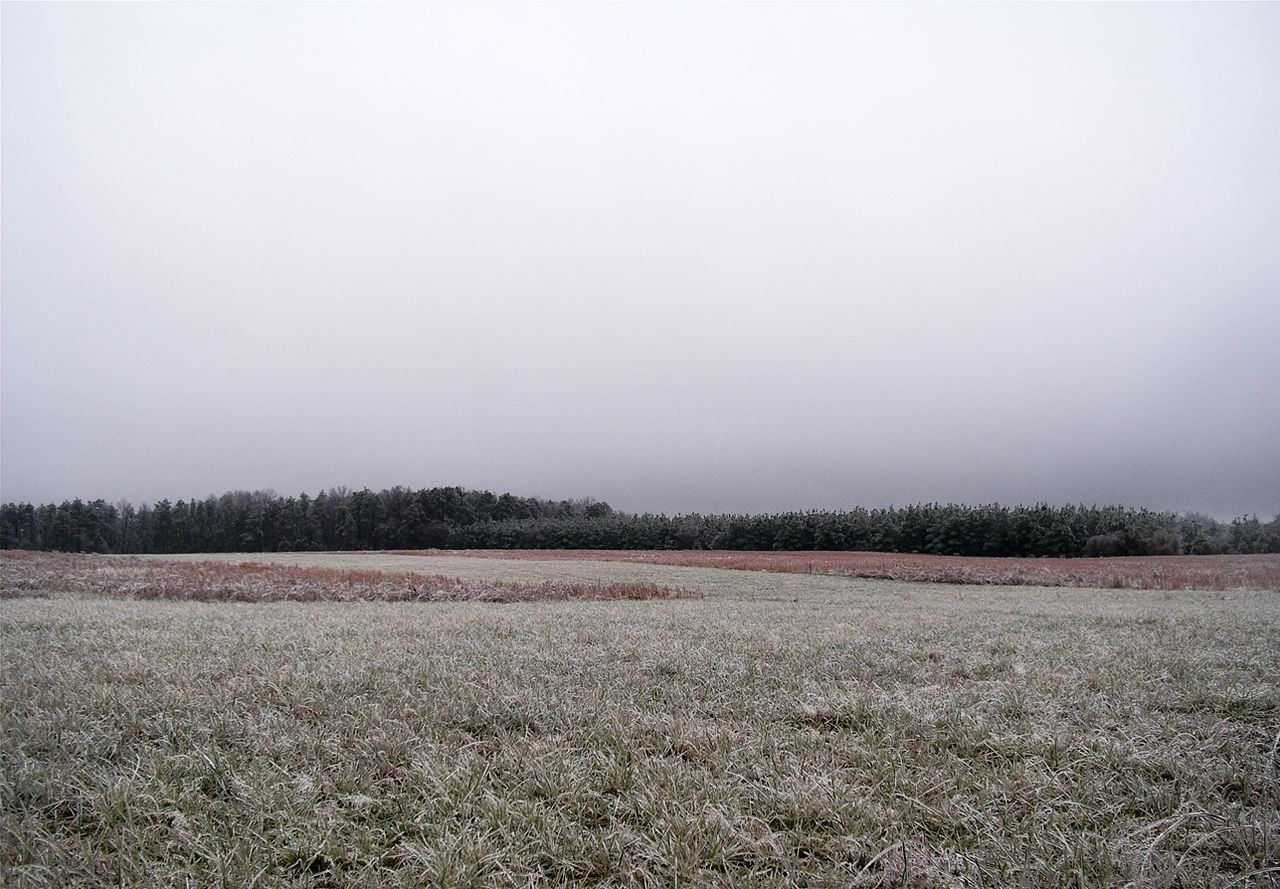
\includegraphics[width=\linewidth]{cloudforms-stratus}
            \captionof{figure}{Photographic reference of stratus clouds \protect\cite{img:cloudforms:stratus}.}
            \label{img:photo:cloudforms-stratus}        
        \end{minipage}        
    \hfill
        \begin{minipage}{0.47\linewidth}
            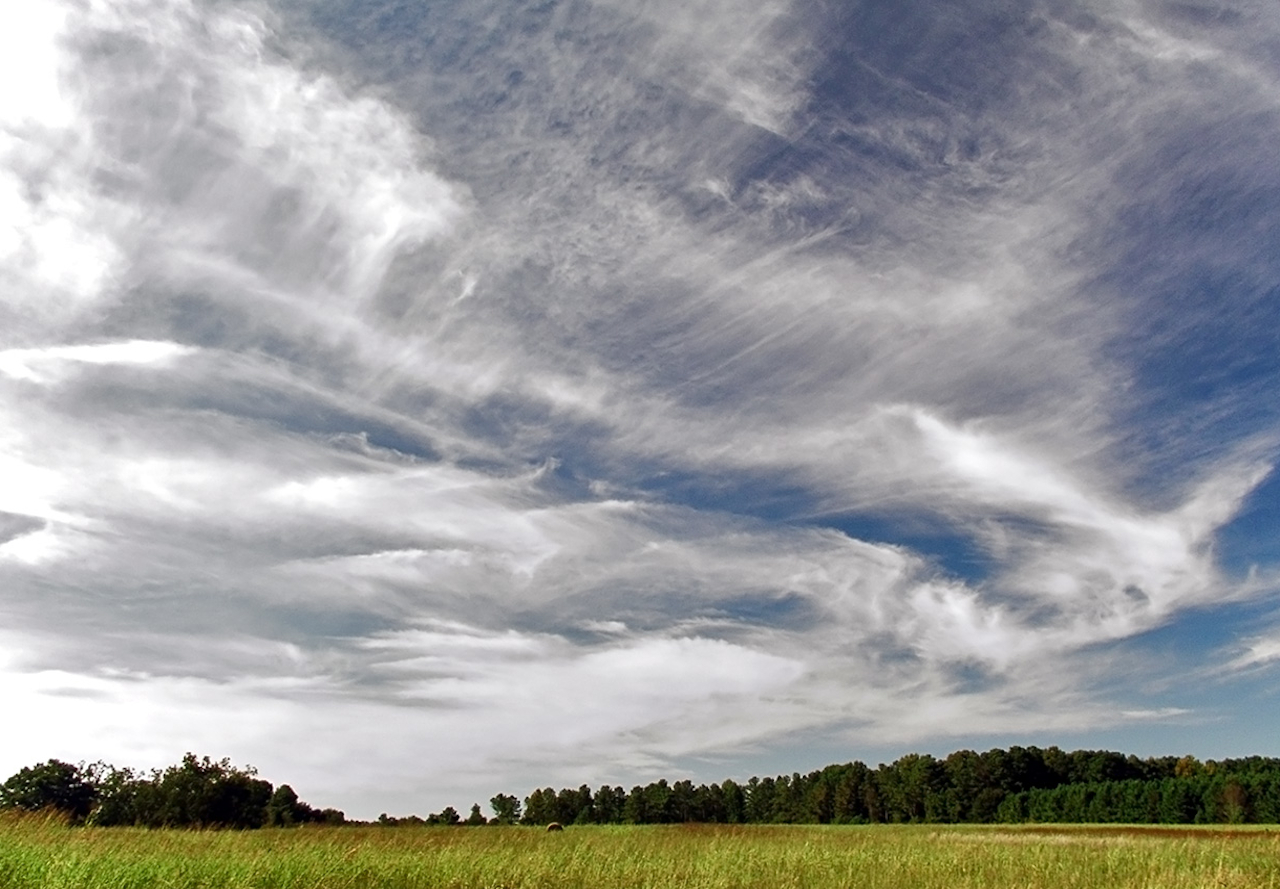
\includegraphics[width=\linewidth]{cloudforms-cirrus}
            \captionof{figure}{Photographic reference of cirrus clouds \protect\cite{img:cloudforms:cirrus}.}
            \label{img:photo:cloudforms-cirrus}        
        \end{minipage}
\end{figure}

\begin{figure}[ht]
    \centering
        \begin{minipage}{0.47\linewidth}
            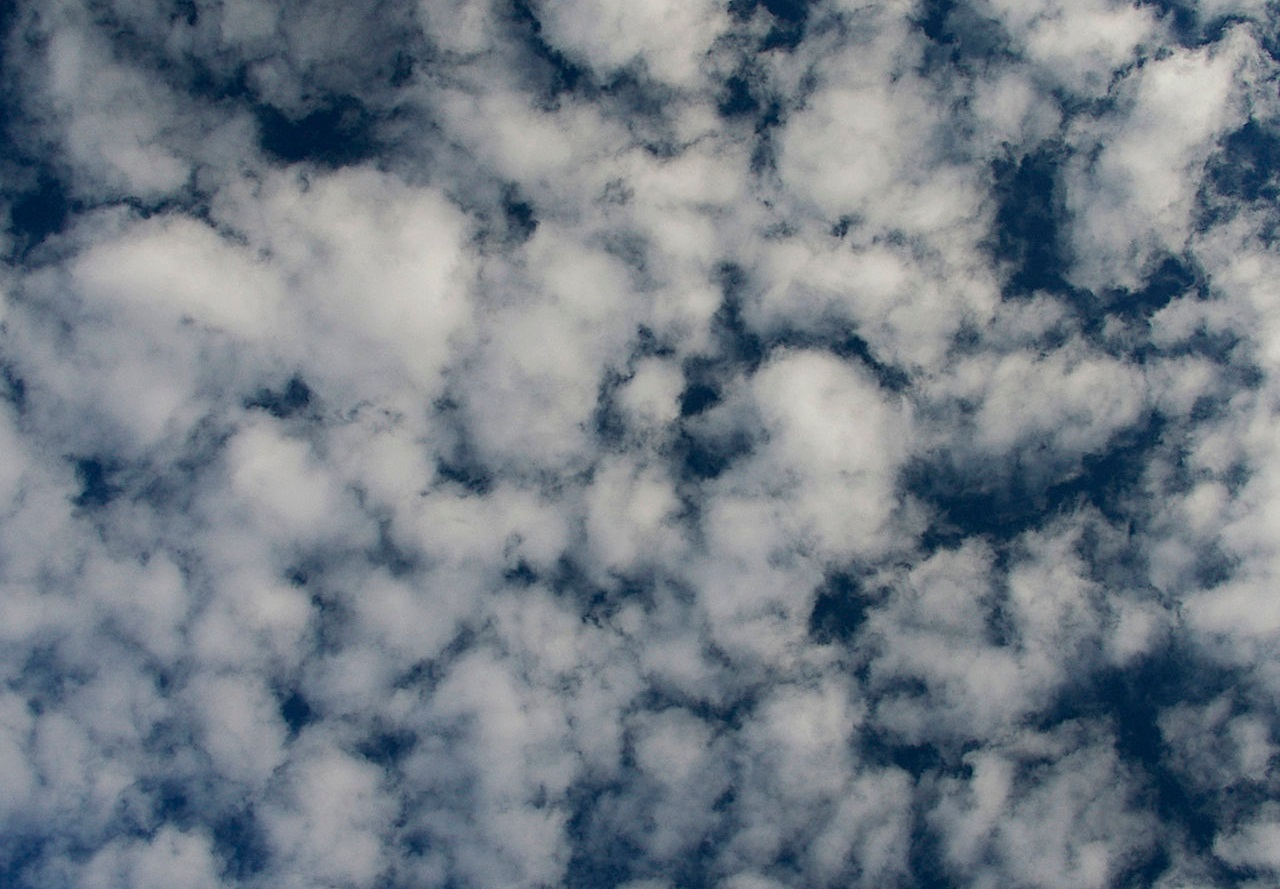
\includegraphics[width=\linewidth]{cloudforms-altocumulus}
            \captionof{figure}{Photographic reference of an altocumulus cloud formation \protect\cite{img:cloudforms:altocumulus}.}
            \label{img:photo:cloudforms-altocumulus}        
        \end{minipage}        
    \hfill
        \begin{minipage}{0.47\linewidth}
            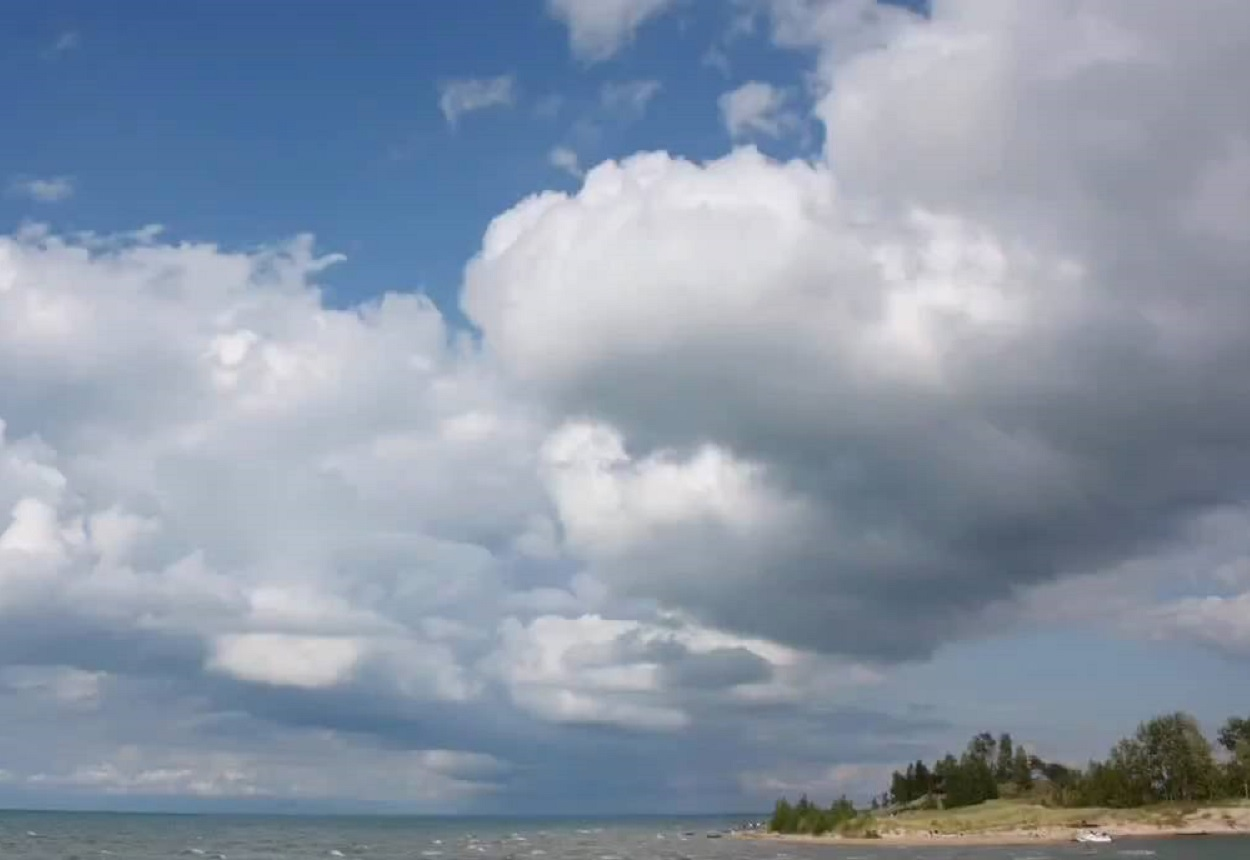
\includegraphics[width=\linewidth]{cloudforms-stratocumulus}
            \captionof{figure}{Photographic reference of stratocumulus cloudscape \protect\cite{img:cloudforms:stratocumulus}.}
            \label{img:photo:cloudforms-stratocumulus}        
        \end{minipage}  
\end{figure}

\subsection{Clouds in games}
\label{section:clouds-in-games}
Depicted in \autoref{img:photo:cloudforms-altocumulus} and \autoref{img:photo:cloudforms-stratocumulus} of \sectionref{section:cloud-types} are clouds of the genus \textit{cumulus}, which translated to English means \textit{heap} or \textit{pile}.
Their distinctive cotton-like look makes them easy to recognize, which is also why they are often used in games as a reference for "normal" clouds. 
\\
In games, the formation as well as the natural composition of clouds are irrelevant, as they are essentially only used for cinematic ambience or as a medium to enhance the atmosphere. This leaves just the rendering technique and performance to worry about.

\subsubsection{Skyboxes}
A widespread solution for representing clouds in games is not rendering them separately at all, but instead using a set of polar sky dome images, also known as the skybox. This is a six-sided cube which is rendered around the whole game world. On each inward looking face of the cube, one of the sky dome images is displayed, creating a seemless sky around the inner side of the box.
\begin{figure}[H]
    \centering
        \begin{minipage}{0.47\linewidth}
            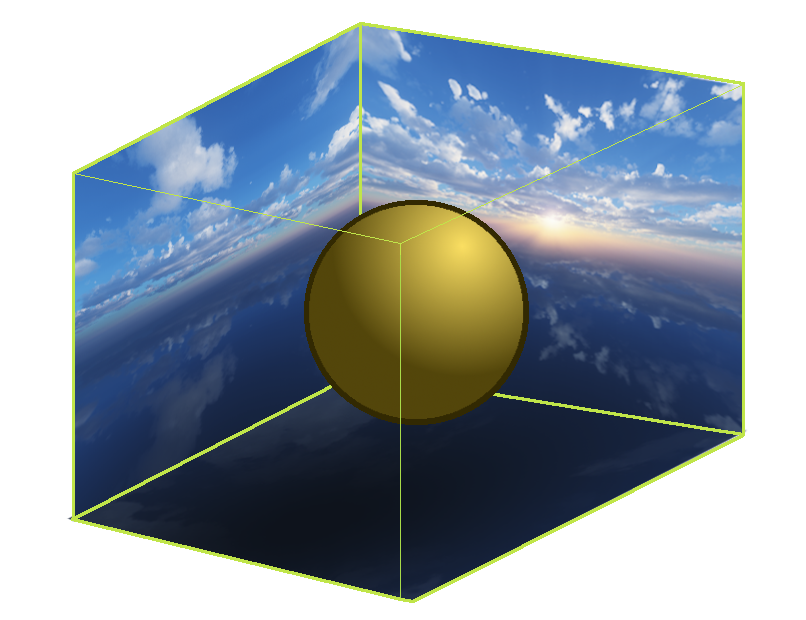
\includegraphics{edits/skybox}
            \captionof{figure}{The skybox cube as it is used in games.}
            \label{img:edits:skybox}
        \end{minipage}
    \hfill
        \begin{minipage}{0.45\linewidth}
            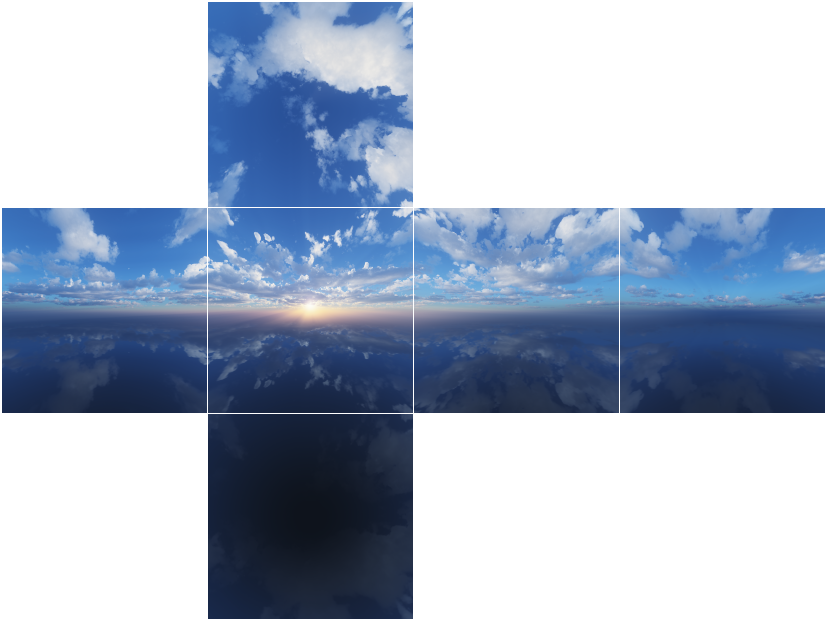
\includegraphics[width=\linewidth]{edits/skybox_layedout}
            \captionof{figure}{The polar sky dome images, folded out.}
            \label{img:edits:skybox_layedout}
        \end{minipage}
\end{figure}

\noindent
Besides rendering the sky, this of course allows clouds to be drawn right into the background. Also, in terms of performance, this is extremely cheap and efficient. On the other hand, it removes the ability for the clouds to move. 
They also have no volumetric body and no way of interaction with the game world whatsoever.
\\
This method does indeed give the scenery a more cloudy look, but what is missing is the "feel", or in other words the motion, interaction and lifelikeness of the clouds.

\subsubsection{Billboards}
Similar to the approach with the skybox, this technique also only uses 2D images of clouds. They are rendered individually and are always facing the camera. This is called \textit{\gls{billboard}ing}.
Now that each cloud is represented by its own game object, having a position in \gls{worldspace} as well as a scale and many other properties, it is possible to animate the clouds. For example, by moving the game objects in a circle around the world, the clouds seemingly "pass by".
\begin{figure}[H]
    \centering
        \begin{minipage}{0.48\linewidth}
            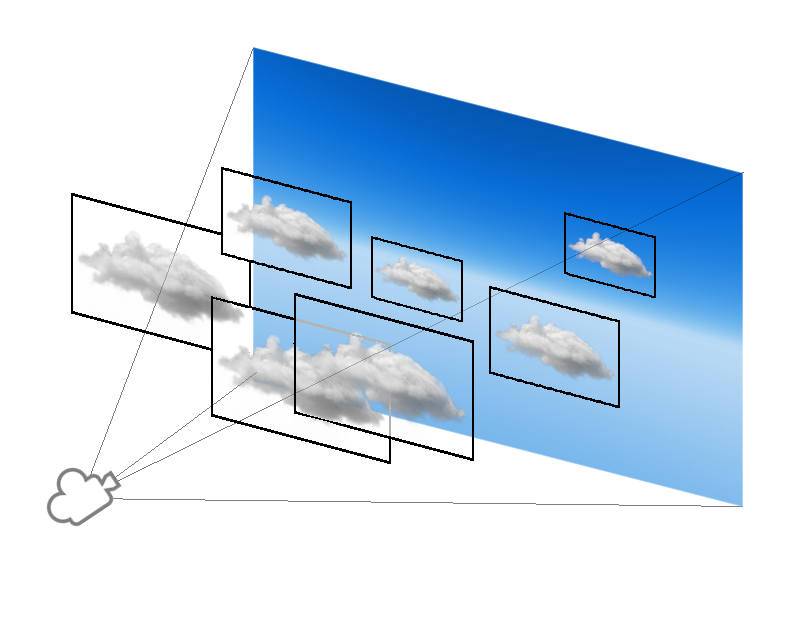
\includegraphics{edits/billboards}
            \captionof{figure}{A collection of 2D cloud billboards facing the camera.}
            \label{img:edits:billboards}
        \end{minipage}
    \hfill
        \begin{minipage}{0.45\linewidth}
            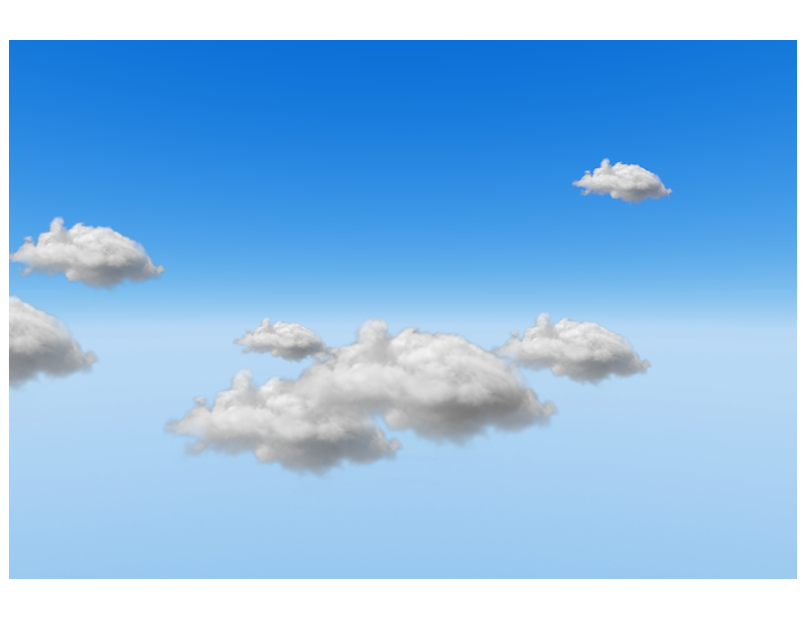
\includegraphics[width=\linewidth]{edits/billboards_rendered}
            \captionof{figure}{The rendered result of the image to the left.}
            \label{img:edits:billboards_rendered}
        \end{minipage}
\end{figure}
\noindent
Due to billboarding, the orientation is already given, making the overall time and effort of this technique quite advantageous to others.
\\
The major flaw of using billboards is of course that they are still 2D images, meaning they cannot really change appearance and therefore, do not evolve at all. 
Still, for many games, this technique suffices in the required diversity of background scenery and does not exceed the allowed performance share for such a task.

\subsubsection{Mesh-based Objects}
It is imaginable to simply use a \gls{polymesh} shaped like a cloud and render that like any other game object. By adding a texture, this would make for some decent looking clouds.
\\
However, the level of detail of such a polymesh is directly connected to the amount of vertices and faces that have to be processed every frame.
As seen in \autoref{img:rendered:cloud-mesh}, there are hundreds of polygons required to merely represent the basic shape of a realistic cloud.
If a similarly complex mesh is to be used for every cloud, a massive overhead is generated for objects that usually only contribute to the background of a game.
\begin{figure}[H]
    \centering
    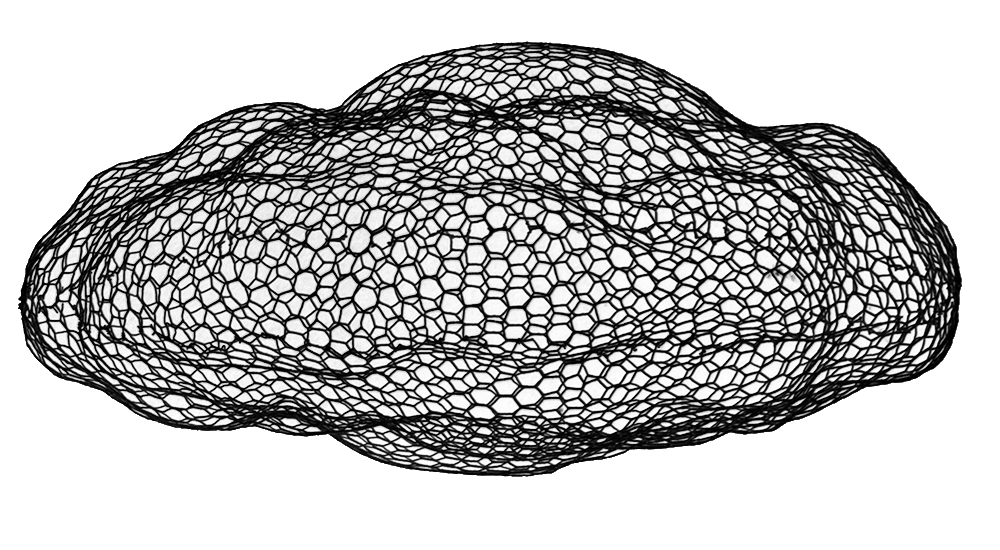
\includegraphics[width=0.5\linewidth]{rendered-cloud-mesh}
    \captionof{figure}{A \gls{polymesh} in the shape of an altocumulus cloud \cite{img:rendered:cloud-mesh}.}
    \label{img:rendered:cloud-mesh}
\end{figure}
\noindent
Apart from the performance impact, this method offers a volumetric, possibly interactable object just like any other 3D model does.
When massively decreasing the polygon count and therefore relinquishing the realistic look, mesh-based objects may be a viable solution for some \gls{lowpoly} games.
Otherwise, it is not reasonable to use this method.

\subsubsection{Volumetric Clouds}
Finally, clouds can be rendered via a technique called \textit{volumetric rendering}. The image below shows volumetric cloudscapes as seen in popular AAA titles.
The method itself is explained in detail in \sectionref{section:volumetric-rendering}.

\begin{figure}[H]
    \centering
    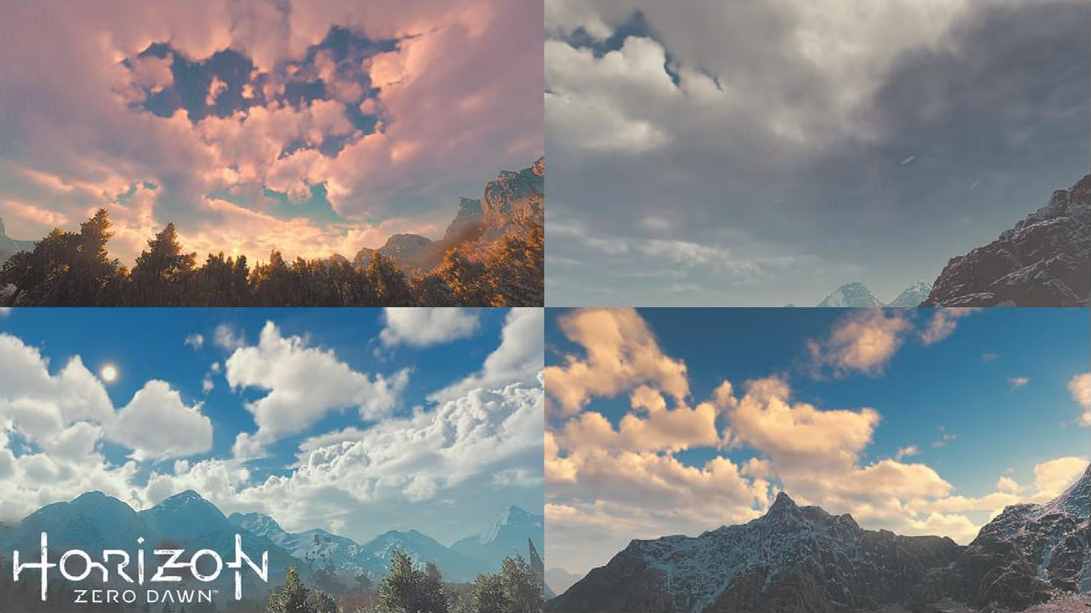
\includegraphics[width=\linewidth]{rendered-clouds-zerodawn}
    \captionof{figure}{Several volumetric cloudscapes from the game \textit{Horizon: Zero Dawn}, drawn in real time \protect\cite{img:rendered:clouds-zerodawn}.}
    \label{img:rendered:clouds-zerodawn}
\end{figure}
\clearpage

\section{Rendering techniques}

\subsection{Volumetric rendering}
\label{section:volumetric-rendering}

\subsubsection{Definition}
\Gls{volumetricrendering} describes a technique for generating a visual representation of data that is stored in a 3D volume. 
This especically comes to use for visual effects that are volumetric in nature, like fluids, clouds, fire, smoke, fog and dust, which all are extremely difficult or even impossible to model with geometric primitives.
\\
In addition to rendering such effects, volumetric rendering has become essential to scientific applications like medical imaging, for which a typical 3D data volume is a set of 2D slice images acquired by a CT (computed tomography) or MRI (magnetic resonance imaging) scanner.
\emptyline
The data volume is also called a \textit{\gls{scalarfield}} or \textit{\gls{vectorfield}}, which associates a scalar value, or \textit{\gls{voxel}}, to every point in the defined space.
This can be imagined like a 3D grid, where each point holds a single number. This number could, for example, represent the density of a cloud at that very point.
A \gls{voxel} may also consist of more than just a single value, but rather a set, like an RGB color.

\subsubsection{Ray Marching with constant step}
To actually render the volume data, a method called \textit{\gls{raymarching}} is used. With it, the surface distance of the volumetric data is approximated by creating a ray from the camera to the object for each fragment processed in the fragment shader. The ray is then extended into the volume of the object and stepped forward until the surface is reached.

\begin{figure}[H]
    \centering
    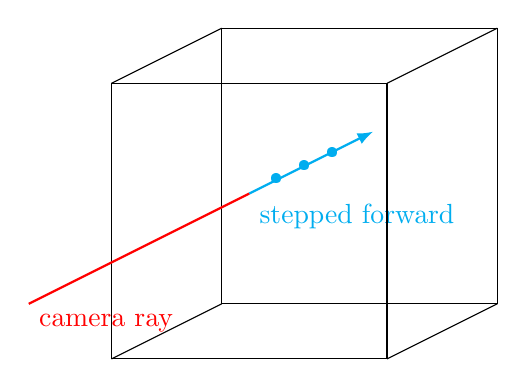
\begin{tikzpicture}[scale=0.7]
        \draw[-{Latex[length=2mm]},thick,cyan] (2.5,3) node[below right]{stepped forward} -- (4.75,4.125);
        \node[cyan] at (3.0,3.25) {\textbullet};
        \node[cyan] at (3.5,3.50) {\textbullet};
        \node[cyan] at (4.0,3.73) {\textbullet};
        
        \draw (0,0) -- (5,0) -- (5,5) -- (0, 5) -- (0, 0);
        \draw (2,1) -- (7,1) -- (7,6) -- (2, 6) -- (2, 1);
        \draw (0,0) -- (2,1); \draw (5,0) -- (7,1); \draw (5,5) -- (7,6); \draw (0,5) -- (2,6); 

        \draw[thick,red] (-1.5,1) node[below right]{camera ray} -- (2.5,3);

    \end{tikzpicture}
    \caption{A ray is created from the camera to the object. From there, it is extended into the volume.}
\end{figure}

\pagebreak
\noindent
In \gls{raymarching}, the algorithm only knows when it has reached the surface, or to be precise when it is inside the actual object volume.
\\
With this information, it is only possible to extend the ray in steps of a predefined length until the inside of the object is reached.
With a constant step, the approximation of the surface distance is exactly as precise as the size of the constant step.
\\
Once the ray is inside the actual volume, the functions returns the distance for this ray.

\begin{figure}[H]
    \centering
    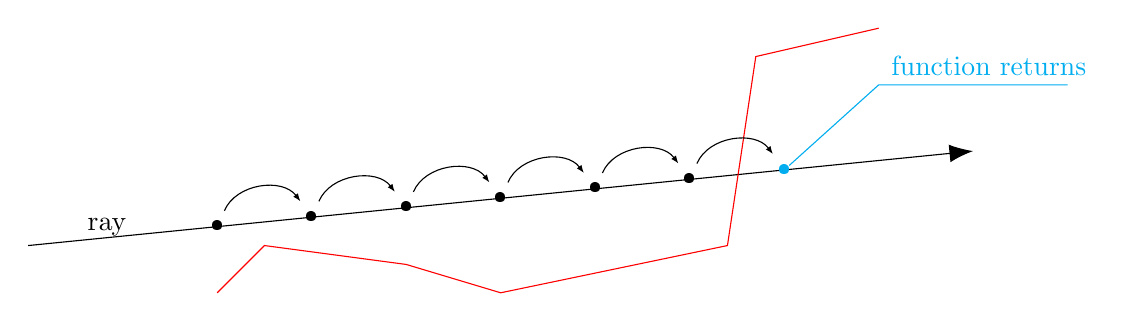
\begin{tikzpicture}[scale=1.2]
        \tikzset{edge/.style = {-{Latex[length=3mm]}}}
        \tikzset{smalledge/.style = {-{Latex[length=1mm]}}}

        % ray
        \draw[edge] (0,2) node[above,sloped,xshift=1cm]{ray} -- (10,3);
        \node (1) at (2,2.2) {\textbullet};
        \node (2) at (3,2.3) {\textbullet};
        \node (3) at (4,2.4) {\textbullet};
        \node (4) at (5,2.5) {\textbullet};
        \node (5) at (6,2.6) {\textbullet};
        \node (6) at (7,2.7) {\textbullet};
        \node[cyan] (7) at (8,2.8) {\textbullet};

        % surf dist
        \draw[red] (2,1.5) -- (2.5,2) -- (4,1.8) -- (5,1.5) -- (7.4,2) -- (7.7,4) -- (9,4.3);

        % ray steps
        \draw[smalledge] (1) edge[bend left=60] node [left]{} (2);
        \draw[smalledge] (2) edge[bend left=60] node [left]{} (3);
        \draw[smalledge] (3) edge[bend left=60] node [left]{} (4);
        \draw[smalledge] (4) edge[bend left=60] node [left]{} (5);
        \draw[smalledge] (5) edge[bend left=60] node [left]{} (6);
        \draw[smalledge] (6) edge[bend left=60] node [left]{} (7);

        % returns text
        \draw[cyan, shorten <=-0.2cm] (7) -- (9,3.7) -- (11,3.7) node[xshift=-1cm,above]{function returns};
        
        \end{tikzpicture}
    \caption{The function returns the evaluated surface distance, the precision of which being directly dependent on the step size.}
\end{figure}

\noindent
An implementation of this algorithm can be seen in \autoref{lst:shader:raymarch:spherehit}. Note that the volume to be rendered in this example is just a simple sphere.
So in order to check if the ray is inside the volume, the function \lstinline[language=HLSL]{sphereHit()} is used.
\begin{lstlisting}[language=HLSL, numbers=left, caption=The function returns true if the ray is inside the volume.,captionpos=b, label=lst:shader:raymarch:constantstep]
bool sphereHit(float3 position) {
    float4 sphere = float4(0, 1, 0, 1);
    return distance(sphere.xyz, position) < sphere.w;
}
\end{lstlisting}

\noindent
\newline 
With that given, the raymarch function is implemented like so:

\begin{lstlisting}[language=HLSL, numbers=left, caption=Ray march function with constant step.,captionpos=b, label=lst:shader:raymarch:spherehit]
fixed4 raymarch(float3 position, float3 direction)
{
    for (int i = 0; i < MAX_STEPS; i++)
    {
        if (sphereHit(position))
            return fixed4(1,0,0,1);
        
        position += normalize(direction) * STEP_SIZE;
    }
    
    return fixed4(0,0,0,1);
}
\end{lstlisting}


\subsubsection{Traditional Ray Marching}
It is obvious to see that, for a constant step ray march to result in an accurate approximation of the surface distance, the step size is required to be relatively small.
This has a direct impact on performance and thus, is not a viable solution for the problem.
\\
In traditional \gls{raymarching}, an optimization for that has been developed. The algorithm does not blindly step forward, but instead tries to get as close to the real distance as possible.
After the volume is reached, the step size is decreased and the ray steps out of the volume again. It then tries to approximate the surface distance by stepping back and forward repeatedly in continuously smaller steps, thus converging towards the exact intersection.
Once the step size falls below a certain threshold, the distance approximation is assumed to be precise enough and the value is returned for that ray march.

\begin{figure}[H]
    \centering
    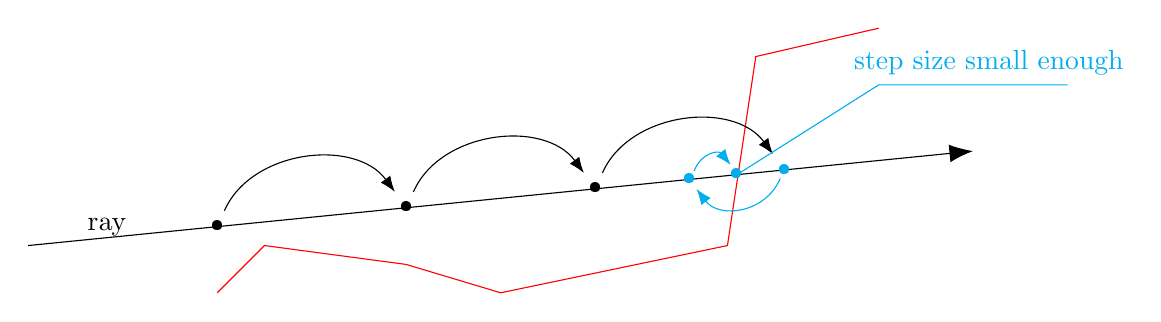
\begin{tikzpicture}[scale=1.2]
        \tikzset{edge/.style = {-{Latex[length=3mm]}}}
        \tikzset{smalledge/.style = {-{Latex[length=2mm]}}}

        % ray
        \draw[edge] (0,2) node[above,sloped,xshift=1cm]{ray} -- (10,3);
        \node (1) at (2,2.2) {\textbullet};
        \node (2) at (4,2.4) {\textbullet};
        \node (3) at (6,2.6) {\textbullet};
        \node[cyan] (4) at (8,2.8) {\textbullet};

        % surf dist
        \draw[red] (2,1.5) -- (2.5,2) -- (4,1.8) -- (5,1.5) -- (7.4,2) -- (7.7,4) -- (9,4.3);

        % reverse nodes
        \node[cyan] (5) at (7,2.7) {\textbullet};
        \node[cyan] (6) at (7.5,2.75) {\textbullet};

        % ray steps
        \draw[smalledge] (1) edge[bend left=60] node [left]{} (2);
        \draw[smalledge] (2) edge[bend left=60] node [left]{} (3);
        \draw[smalledge] (3) edge[bend left=60] node [left]{} (4);

        % rey reverse steps
        \draw[smalledge,cyan,shorten >=-0.1cm,shorten <=-0.1cm] (4) edge[bend left=60] node [left]{} (5);
        \draw[smalledge,cyan,shorten >=-0.1cm,shorten <=-0.1cm] (5) edge[bend left=60] node [left]{} (6);

        % close enough
        \draw[cyan, shorten <=-0.2cm] (6) -- (9,3.7) -- (11,3.7) node[xshift=-1cm,above]{step size small enough};
        
        \end{tikzpicture}
    \caption{The function returns the distance for this ray, which is the amount of steps times the step size.}
\end{figure}

\begin{lstlisting}[language=HLSL, numbers=left, caption=Traditional ray march function with converging surface distance approximation.,captionpos=b, label=lst:shader:raymarch:traditional]
fixed4 raymarch(float3 position, float3 direction)
{
    float stepSize = STEP_SIZE;
    float dirMultiplier = 1;
    for (int i = 0; i < MAX_STEPS; i++)
    {
        if (stepSize < MINIMUM_STEP_SIZE)
            return fixed4(1,0,0,1);

        if (sphereHit(position)) {
            // reduce step size by half and invert marching direction.
            stepSize /= 2;
            dirMultiplier = -1;
        } else {
            dirMultiplier = 1;
        }
        
        position += normalize(direction) * stepSize * dirMultiplier;
    }
    
    return fixed4(0,0,0,1);
}
\end{lstlisting}
\clearpage

\section{Common Algorithms}

\subsection{Noise Generation}
\label{section:noise-generation}
Nature's unpredictability and plays a big role in the diversity and appearance of cloudscapes. In shaders, an approach to that \textit{randomness} is used called \textit{\gls{noise}}.
In order to be able to implement random \gls{noise}, several important topics need to be looked into. It is best to start with randomness in computer science and how it is handled inside a shader program.

\subsubsection{Random Numbers}
As expected, there is no magic function which returns a pure random number inside the seemingly predictable and rigid code environment.
So the question how to generate randomness arises. 
\\
For this, the function $rnd(x) = fract(sin(x))$ is inspected, where $fract(x) = x - floor(x)$.

\begin{figure}[H]
    \centering
    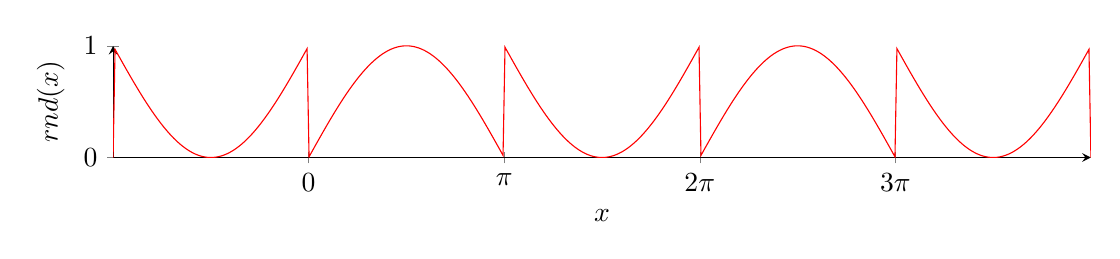
\begin{tikzpicture}[scale=1.0]
        \begin{axis}[
            samples=500,
            domain=-1*pi:4*pi,
            axis lines=left,
            xlabel=$x$,
            ylabel={$rnd(x)$},
            height=3cm,
            width=14cm,
            ytick={0,1},
            xtick={0,pi,2*pi,3*pi},
            xticklabels={$0$,$\pi$,$2\pi$,$3\pi$}
            ]
        \addplot[red] plot (\x, { sin(\x*1 r) - floor(sin(\x*1 r)) });
        \end{axis}
    \end{tikzpicture}
    \caption{Random numbers with the fractional value of sine of x.}
\end{figure}

\noindent
The sine values fluctuate between $-1$ and $1$, but with $fract$, only the fractional part is evaluated, turning the negative values in positive ones.
This effect can be used to get some pseudo-random values by "compressing" the function vertically or in other words, by increasing the frequency of the sine wave.
\\
The next figure displays the function $rnd(x) = fract(sin(x) * 10000)$.

\begin{figure}[H]
    \centering
    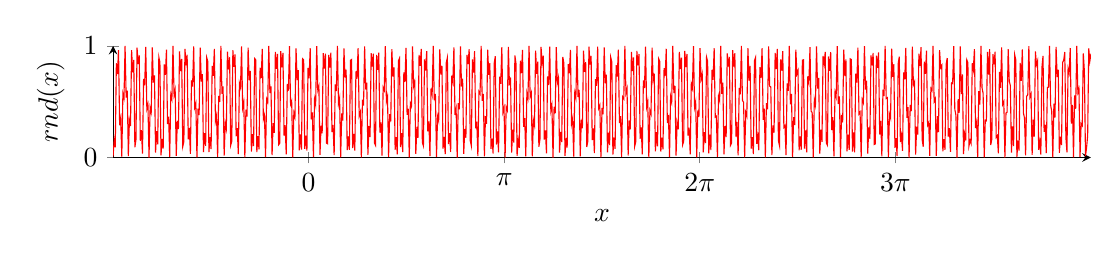
\begin{tikzpicture}[scale=1.0]
        \begin{axis}[
            samples=899,
            domain=-1*pi:4*pi,
            axis lines=left,
            xlabel=$x$,
            ylabel={$rnd(x)$},
            height=3cm,
            width=14cm,
            ytick={0,1},
            xtick={0,pi,2*pi,3*pi},
            xticklabels={$0$,$\pi$,$2\pi$,$3\pi$}
            ]
        \addplot[red] plot (\x, { sin(\x*10000 r) - floor(sin(\x*10000 r)) });
        \end{axis}
    \end{tikzpicture}
    \caption{Random numbers with the fractional value of sine of x multiplied by 10000.}
\end{figure}

\noindent
It is clearly visible that the function $rnd(x)$ became chaotic and seemingly random. However, it is noteworthy that $rnd(x)$ is still a deterministic function, which means for example $rnd(1.0)$ is always going to return the same value.
\clearpage

\section{Project management}

\subsection{Schedule}
The time frame of the semester spans over exactly 16 weeks. Being worth 4 ECTS points, this project assumes a maximum work load of 8 hours per week, resulting in a total of 128 hours. 
\vspace{\baselineskip}
\\
Over the course of the term, the project will be split into four primary task groups, namely organization, research, prototyping and finalization.
Put into relation with the duration of the project, the estimated schedule looks like this:
\vspace{\baselineskip}

\begin{ganttchart}[
    vgrid={dotted},
    hgrid={draw=black!50, dotted},
    bar/.append style={fill=lightgray},
    x unit=0.65cm,
    milestone node/.append style={fill=orange}
    ]{1}{16}
    \gantttitle{Work weeks}{16} \\
    \gantttitlelist{1,...,16}{1} \\
    \ganttbar{Organization}{1}{4} \\
    \ganttmilestone{Specification finished}{4} \\
    \ganttgroup{Documentation}{5}{15} \\
    \ganttbar{Research}{5}{11} \\
    \ganttbar{Prototyping}{7}{15} \\
    \ganttmilestone{Prototype 1 finished}{9} \\
    \ganttmilestone{Prototype 2 finished}{11} \\
    \ganttmilestone{Prototype 3 finished}{15} \\
    \ganttbar{Finalizing}{16}{16}
\end{ganttchart}

\vspace{\baselineskip}
\begin{flushleft}
The milestones \emph{Prototype finished} for prototypes 1, 2, and 3 are referring to the prototypes about \gls{volumetric}, \gls{noise} and \gls{raymarching}, respectively.
\\
\vspace{\baselineskip}
During research and prototyping, the documentation will be continuously updated.
\\
For each task group, the following distribution of time and effort is estimated:
\newline
\newline
\begin{tabular}{|c|c|}
    \hline
    \textbf{Task group}  & \textbf{Predicted effort}\\ \hline
    Organization        & 10\%                      \\ \hline
    Research            & 35\%                      \\ \hline
    Prototyping         & 50\%                      \\ \hline
    Finalizing          & 5\%                       \\ \hline
\end{tabular}
\end{flushleft} 

%==============================================================

\clearpage
\subsection{Project Organization}
A meeting will be held bi-weekly to discuss the progress of the project, possibly arisen issues as well as planned work for the upcoming two weeks.
\vspace{\baselineskip}
\newline
\noindent Mandatory participants are:
\vspace{\baselineskip}
\newline
\noindent\begin{tabular}{|l|l|}
    \hline
    \textbf{Name}       & \textbf{Role}         \\ \hline
    Matthias Thomann    & Author                \\ \hline
    Prof. Urs Künzler   & Tutor and reviewer    \\ \hline
\end{tabular}

\vspace{\baselineskip}
\noindent Should a physical meeting be impossible for some reason, an online meeting via Microsoft Teams will be held instead.

%==============================================================

\subsection{Project Results}

\subsubsection{Documentation}
The following documents must be submitted for grading:
\begin{itemize}
    \item Requirement specification
    \item Project documentation indcluding:
    \begin{itemize}
        \item Conceptual formulation
        \item Comparison and details of methods and algorithms
        \item Details of implementation
        \item Result report
    \end{itemize}
\end{itemize}

\subsubsection{Implementation of the Shader}
The Unity project, including the implemented shader code, will be managed and stored in the given Gitlab repository\cite{gitlab}. This will also serve as a form of submission for grading.

\subsubsection{Presentation}
A presentation will be held on the second last friday of the term, June 5th, 2020.

\subsubsection{Submission terms}
The project must be submitted in digital form on the last friday of the term, June 12th, 2020 before 12pm.
\clearpage

\section{Prototypes and Results}

\subsection{Disclaimer}
\subsubsection{Completed Prototypes}
While researching the topic and experimenting with some dummy shaders, it came clear that "\gls{volumetricrendering}" and "\gls{raymarching}" are interchangeable in this matter.
Therefore, only two kinds of prototyping have been developed. This change is explained in detail in \sectionref{section:projectmanagement:goals}.

\subsubsection{Dimensions}
All of the following documented procedures and algorithms were prototyped and implemented in 3D, but for the matter of explanation, it is described and visualized in 2D.

\subsubsection{Unity Variables}
The following sections will list code snippets, in which all variables prefixed with an underscore are shader variables exposed to the Unity Editor. This way, they can be changed externally while running the shader code, allowing for convenient debugging.
They are from here on out referred to as \textit{\gls{parameters}}.

\clearpage
\subsection{First Draft}
The first drafts of prototypes created during this project all revolve around volumetric rendering. 
Instead of using a \gls{sdf} and evaluating the distance each step, a noise function was used to simulate the \textit{mass} of the cloud. 
The primary issue was to get the cube transparent where the noise function would return a number close to 0.0 and to color it where the number would be close to 1.0.
The approach for solving this issue is done by sampling the cloud's density.

\subsubsection{Density sampling}
Like in \gls{volumetricrendering}, for each pixel fragment, a ray is cast from the fragment into the cube and extended along the view direction for that fragment.
Usually, the algorithm can stop for a given ray if the \gls{sdf} returns a small enough distance, meaning the ray has hit a surface of the volume. However, it is different in the case with clouds, where the volume is \textit{\gls{translucent}} at most points.
\\
To account for that, the ray does not stop until the end of the container cube is reached. It samples the density $N$ times along its path and returns the sum of those samples, giving an approximate qualifier for how dark this fragment should be.

\begin{figure}[H]
    \centering
    \begin{tikzpicture}[scale=1.2]
        \tikzset{edge/.style = {-{Latex[length=3mm]},shorten >= -4pt}}
        \tikzset{shortedge/.style = {-{Latex[length=3mm]},shorten <=-4pt,shorten >= -4pt}}
        \tikzset{icon/.style = {font=\Large}}

        % icons
        \node[icon,rotate=35,anchor=west] (cam) at (0, 0) {\faVideoCamera};

        % clouds
        \node[cloud, cloud puffs=15.7, minimum width=5cm, minimum height=3.5cm, align=center, draw] (cloud) at (4.5, 3.5) {};
        \node[cloud, cloud puffs=15.7, minimum width=2cm, minimum height=1.5cm, align=center, draw] (cloud) at (5.0, 1.1) {};
        \node[cloud, cloud puffs=15.7, minimum width=3cm, minimum height=2.0cm, align=center, draw] (cloud) at (0.2, 3.5) {};
        \node[cloud, cloud puffs=15.7, minimum width=1.5cm,minimum height= 1cm, align=center, draw] (cloud) at (1.75, 0.9) {};

        % outer point
        \node (pOut) at (7, 5.25) {};
        \draw[red, edge] (cam) -- (pOut) node[midway,above,sloped,xshift=-3cm] {};

        % cloud points
        \node[red] (p1) at (1.5, 1.125) {\textbullet};
        \node (p2) at (2.5, 1.875) {\textopenbullet};
        \node[red] (p3) at (3.5, 2.625) {\textbullet};
        \node[red] (p4) at (4.5, 3.375) {\textbullet};
        \node[red] (p5) at (5.5, 4.125) {\textbullet};

        \node[red, yshift=0.4cm] at (p1) {$p_1$};
        \node[red, yshift=0.4cm] at (p2) {$p_2$};
        \node[red, yshift=0.4cm] at (p3) {$p_3$};
        \node[red, yshift=0.4cm] at (p4) {$p_4$};
        \node[red, yshift=0.4cm] at (p5) {$p_5$};


        \end{tikzpicture}
    \captionof{figure}{Density sampler ray with $N = 5$.}
    \label{img:tikz:prototypes:densitysampling}
\end{figure}

\noindent
Understandably, the bigger clouds in \autoref{img:tikz:prototypes:densitysampling} represent higher return values of the noise function, meaning denser areas.
For the displayed ray, the values for points $p_1, p_3, p_4$ and $p_5$ are accumulated and used as a qualifier to color the fragment. In this case, a rather dark tone would be used.
\\
It is notable that $N$ has a linear impact on the performance, so it should be chosen carefully.
\emptyline
While marching along the ray, the step size is not constant but instead calculated: \\
$ d_{step} = \frac{d_{box}}{N}$, where $d_{box}$ is equal to the total distance the ray travels while inside the box. To determine $d_{box}$, an \gls{aabb} (AABB) intersection test \cite{online:aabb} has to be done with the container cube and the ray.

\begin{figure}[H]
    \centering
    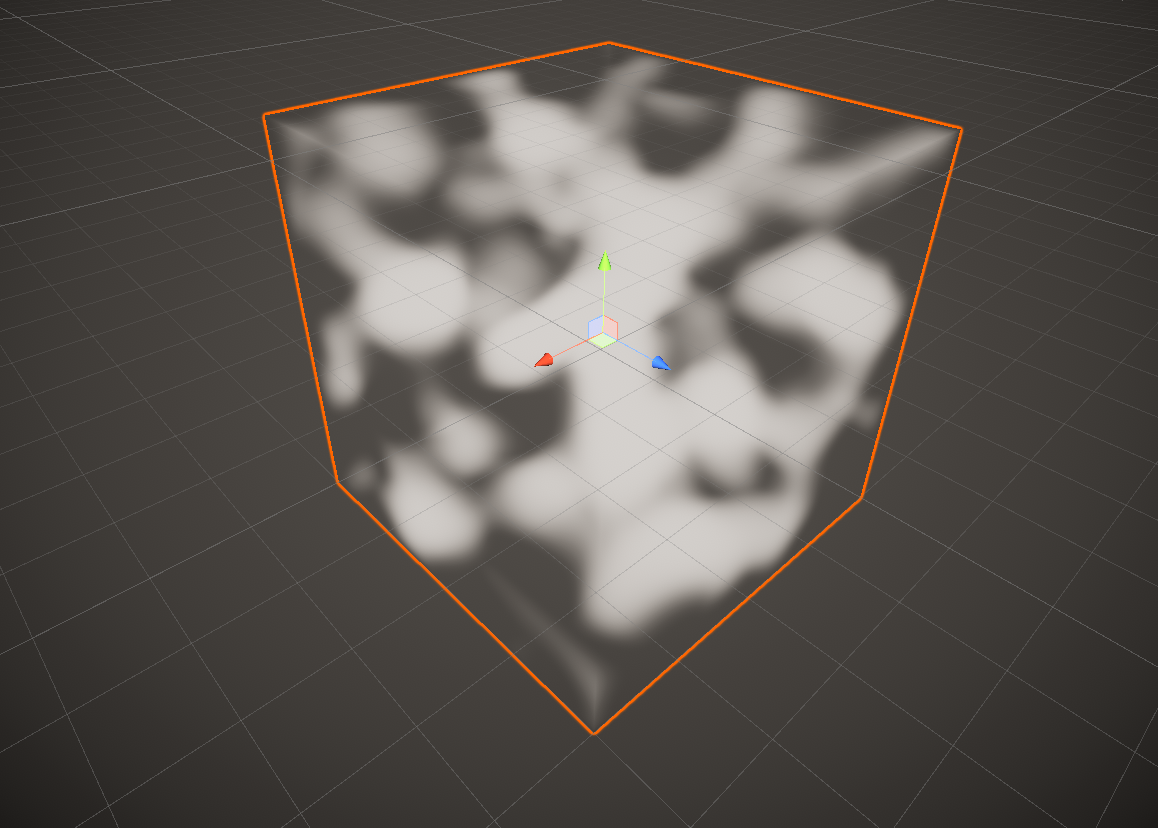
\includegraphics[width=\linewidth]{unity captures/prototype1.PNG}
    \captionof{figure}{Prototype: Rendered image of sampled density based on 3D Perlin noise.}
    \label{img:captures:prototype1}
\end{figure}

\noindent
With this first try, a Perlin noise function was sampled. The returned value had to be normalized in a range of $[0, 1]$ in order for it to be used as alpha value of the color.

\subsubsection{Normalizing Density}
This is where the exponential function $exp(x) = e^{-x}$ comes in, which (when clamped between 0 to 1) converts very low values to 1.0 and higher values will converge towards 0.0.

\begin{figure}[H]
    \centering
    \begin{minipage}{0.47\linewidth}
        \begin{tikzpicture}
            \begin{axis}[
                axis lines=center,
                samples=50,
                xmin=-0.5,
                xmax=4.5,
                ymin=-0.2,
                ymax=1.2,
                xlabel={$x$},
                ylabel={$y$},
                xlabel style={below right},
                ylabel style={above left},
                height=4cm,
                width=8cm,
                ytick={0,1},
                xtick={0,1,2,3,4},
                ]
    
                \addplot[red] plot (\x, { exp(-\x)) });
            \end{axis}
        \end{tikzpicture}
        \captionof{figure}{Exponential function $exp(x) = e^{-x}$.}
        \label{img:math:exp}
    \end{minipage}        
    \hfill
    \begin{minipage}{0.47\linewidth}
        \begin{tikzpicture}
            \begin{axis}[
                axis lines=center,
                samples=50,
                xmin=-0.5,
                xmax=4.5,
                ymin=-0.2,
                ymax=1.2,
                xlabel={$x$},
                ylabel={$y$},
                xlabel style={below right},
                ylabel style={above left},
                height=4cm,
                width=8cm,
                ytick={0,1},
                xtick={0,1,2,3,4},
                ]
    
                \addplot[red] plot (\x, { 1 - exp(-\x)) });
            \end{axis}
        \end{tikzpicture}
        \captionof{figure}{Inverted exponential function $exp'(x) = 1 - e^{-x}$.}
        \label{img:math:exp1}       
    \end{minipage}
\end{figure}

\noindent
When inverting $exp(x)$, the function $exp'(x)$ returns a value that can be directly used for the transparency of the cloud. The denser it gets, the more opaque it will be.

\clearpage
\subsection{Improving Noise}
After further experimenting with the noise sampling function, the idea arose to combine Perlin and Voronoi noise, which hopefully would create a more distinguished, random pattern.
The final sampling function simply multiplies both noise values at a given point \lstinline[language=HLSL]{position}, masking them with each other. 

\begin{lstlisting}[language=HLSL, numbers=left, caption=Implementation of a density sampling function., label=lst:shader:prototype:sampledensity]
float sampleDensity(float3 position) {
  float3 vpos = position * _VoronoiScale + _VoronoiOffset;
  float3 ppos = position * _PerlinScale + _PerlinOffset;
  float vd = fbmVoronoi(vpos, _VoronoiOctaves, _VoronoiPersistence));
  float pd = fbmPerlin(ppos, _PerlinOctaves, _PerlinPersistence));
  
  vd = max(0, vd - _VoronoiDensityThreshold) * _VoronoiDensityMultiplier;
  pd = max(0, pd - _PerlinDensityThreshold) * _PerlinDensityMultiplier;
  
  // fixed boost for density by factor 2
  float density = vd * pd * 2.0;
  return density;
}
\end{lstlisting}

\noindent
By adjusting some of the \gls{parameters} and increasing the octaves of both noises, a more patchy and cloudy look can be achieved at the cost of performance.

\begin{figure}[H]
    \centering
    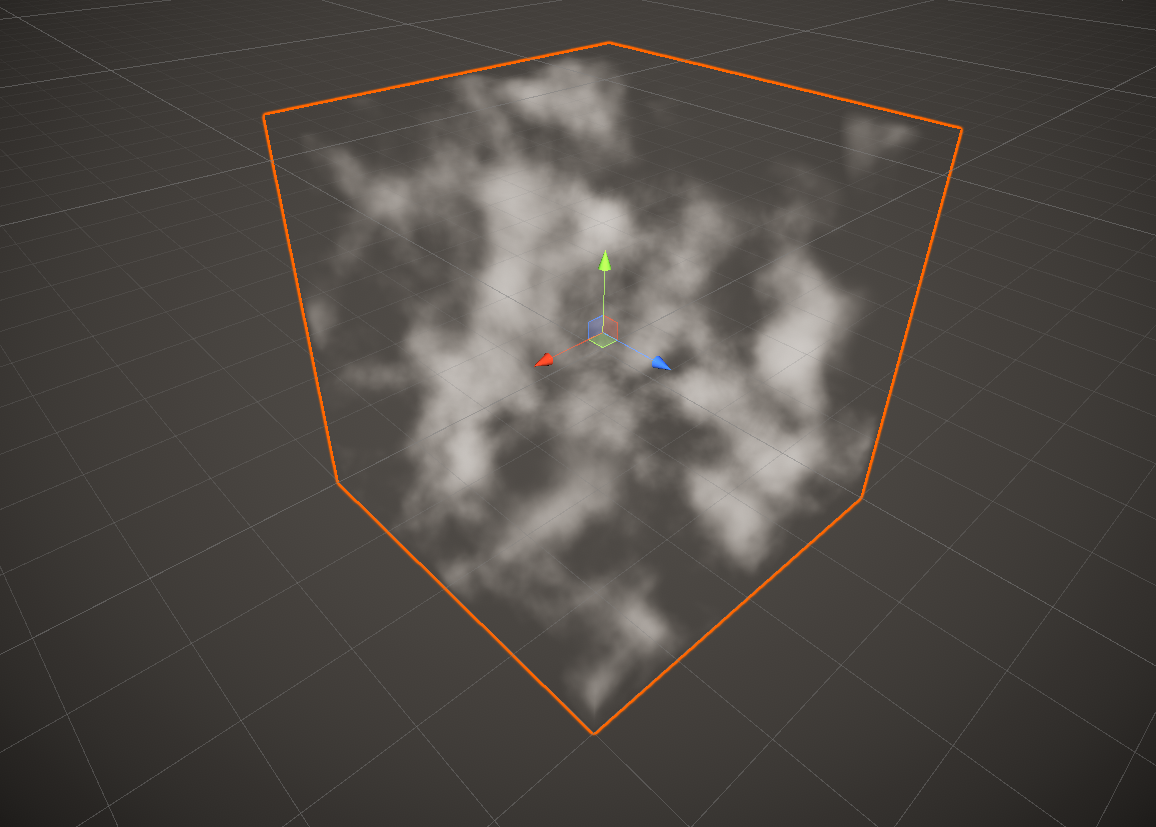
\includegraphics[width=\linewidth]{unity captures/prototype2.PNG}
    \captionof{figure}{Prototype: Rendered image of sampled density based on mixed noises.}
    \label{img:captures:prototype2}
\end{figure}

\clearpage
\subsection{Light Transmittance and Light Scattering}
One of the more prominent lighting features of clouds is its translucency. This phenomenon displays how light bounces and scatters inside the matter, then exits at a different point. This is also called \textit{\gls{sss}} (SSS).
It results in illuminated areas where the clouds are thinner, giving it that milky look and "glow" on the outer edge. In nature, \gls{sss} is a very complex and computationally demanding process. For computer graphics however, it is often either simplified or substituted with some other algorithm that produces a similar outcome at lower performance cost.

\subsubsection{Sunlight Forward Scattering}
When approaching the implementation of \gls{sss} and directional lighting, it seemed most reasonable to start with the sun being visible behind the clouds, or at least shining through them.
This implies finding a way to illuminate clouds that cover the sun. In the context of this project, it is called \textit{\gls{sunlighttransmittance}} or \textit{\gls{sunlightforwarding}}, since it is not a variant of SSS but rather an approximation.
\\
After some consideration and brainstorming, the following method was chosen to solve the issue:

\begin{figure}[H]
    \centering
    \begin{tikzpicture}[scale=1.2]
        \tikzset{edge/.style = {-{Latex[length=3mm]},shorten >= -4pt}}
        \tikzset{shortedge/.style = {-{Latex[length=3mm]},shorten <=-4pt,shorten >= -4pt}}
        \tikzset{line/.style = {shorten >=-4pt}}
        \tikzset{icon/.style = {font=\Large}}

        % icons
        \node[icon,rotate=35,anchor=west] (cam) at (0, 0) {\faVideoCamera};
        \node[icon] (light) at (8, 6) {\faLightbulbO};
        \node at (8, 6.5) {light source};

        % clouds
        \node (cloud) at (4.0, 5.2) {};
        \node[cloud, rotate=-15, cloud puffs=15.7, cloud, minimum width=3.5cm, minimum height=2.2cm, align=center, draw] (cloud) at (cloud) {};

        % screen space
        \draw (1,1) -- (5,0) -- (5,3);

        % rays
        \node[red] (p1) at (3, 2.25) {\ding{53}};
        \node[red] (st1) at ($(p1) + (0.5, -0.2)$) {$st_2$};

        \node[cyan,mark=x] (c1) at (2.4, 2.4) {\ding{53}};
        \node[cyan] (st2) at ($(c1) + (-0.5, 0.2)$) {$st_1$};

        \node (p2) at (5, 3.75) {};
        \node (c2) at (4, 4) {};
        \node[cyan] (c3) at (4.9, 4.9) {\textbullet};

        \draw[red, line] (cam) -- (p1);
        \draw[red, line, loosely dashed] (p1) -- (p2);
        \draw[red, edge, loosely dashed] (p2) -- (light);
        
        \draw[cyan, line] (cam) -- (c1);
        \draw[cyan, line, loosely dashed] (c1) -- (c2);
        \draw[cyan, edge, loosely dashed] (c2) -- (c3);

        % rest of screen space
        \draw (5,3) -- (1,4) node[midway,above,sloped,xshift=-1cm] {screen space} -- (1,1);

        \end{tikzpicture}
    \captionof{figure}{Sunlight transmittance sampling.}
    \label{img:tikz:prototypes:sunlight}
\end{figure}

\noindent
When ray casting, both the fragment's and the light source's screen-space position is calculated. Those are two-dimensional coordinates relative to the screen that the camera renders to.
Now if the distance $d = \norm{\overrightarrow{st_1 st_2}} < t$, with $t$ being some threshold, a portion of the sun's color is added to the fragment's color, relative to how small $d$ is.
\\
It is noteworthy that when calculating the screen-space position, the depth value gets lost. Therefore, theoretically, the clouds would be illuminated when $d < t$ even if the sun is in front of the clouds.
Given this is almost never the case in games and weather simulations, that particular issue is neglected.
\\
Also, instead of evaluating the distance $d$, the intermediate angle of both vectors could also be used to avoid calculating the screen-space position, giving $d = cos^{-1}\left(\overrightarrow{v_{cloud}} * \overrightarrow{v_{light}}\right)$.

\begin{figure}[H]
    \centering
    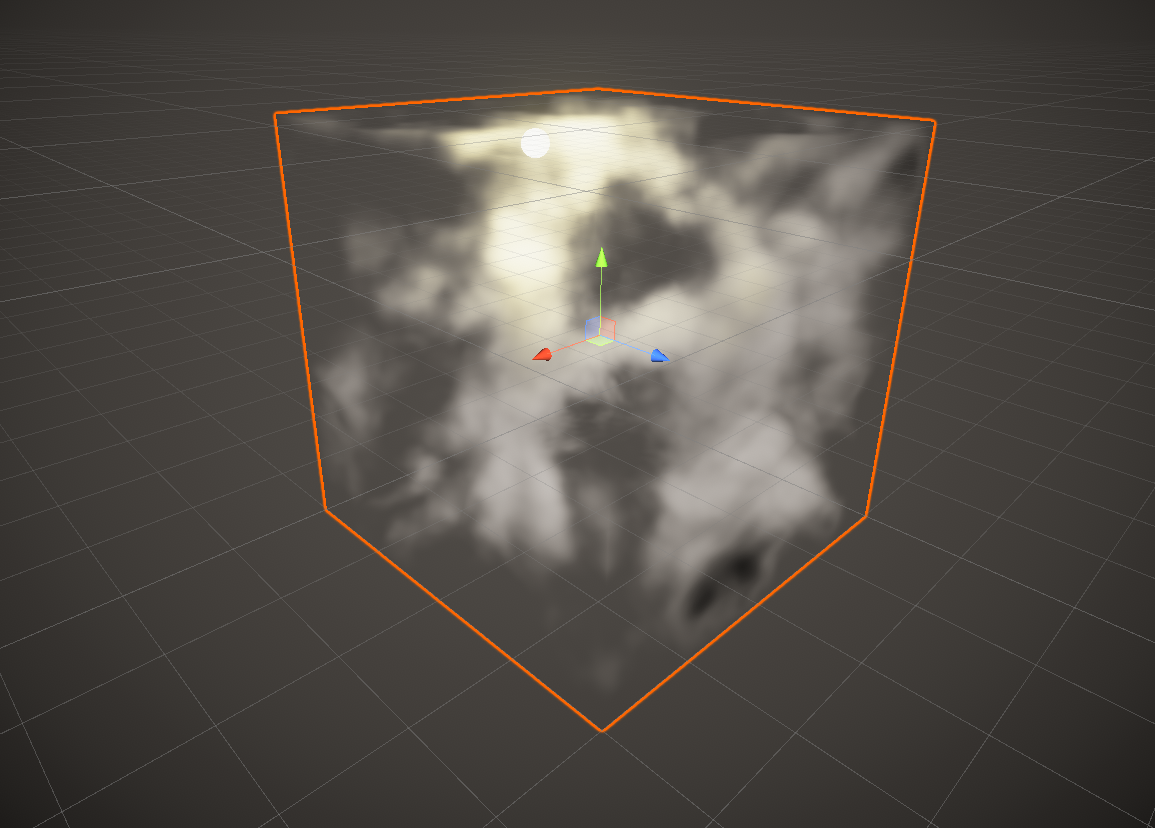
\includegraphics[width=\linewidth]{unity captures/prototype4.PNG}
    \captionof{figure}{Prototype: Rendered image of sunlight transmittance.}
    \label{img:captures:prototype3}
\end{figure}

\noindent
Behind the cube in \autoref{img:captures:prototype3} is a sphere object placed, representing the sun. The sunlight is indeed shining through the clouds, but there are still some minor flaws with the implementation.
For example, some clouds are completely illuminated, making them too bright where the cloud would be too dense for the light to pass through.
\emptyline
The following code snippet shows the implementation of the sunlight transmittance mechanism. The \lstinline[language=HLSL]{density} variable is the one evaluated in \autoref{lst:shader:prototype:sampledensity}.

\begin{lstlisting}[language=HLSL, caption=Implementation of a sunlight transmittance mechanism., label=lst:shader:prototype:sunlighttransmittance]
float cloudDensity = exp(-density);

float projectedSunDistance = length(
  worldToScreenPos(_SunPosition) - worldToScreenPos(worldPosition));

float sunTransmittance = 1 - pow(
  smoothstep(0.01, _SunLightScattering,projectedSunDist), _SunLightStrength);

fixed3 sunColor = sunTransmittance * _LightColor0.xyz * cloudDensity;
\end{lstlisting}

\noindent
Like in other prototype code listings, there are some \gls{parameters} to play with. The sunlight strength or the sunlight range (in screen space) can both be adjusted, for example.
\\
The idea of multiplying by \lstinline[language=HLSL]{cloudDensity} on line 9 was to fix the previously described flaw of clouds being too bright. 

\clearpage
\subsubsection{Directional light}
Another challenging part during prototyping was directional light on surfaces facing the sun. Usually in \gls{raymarching}, a \gls{surfacenormal} estimation is done using the gradient.
This works well if there is only one point of interest (like a ray-surface intersection point), but as already mentioned before, the ray does not stop sampling points until it reaches the end of the container cube.
\\
So instead of calculating normals for each sample point, another ray is cast from the sample point towards the sun.
Along its path, the density is sampled again $L$ times in constant steps. With the lack of an official term, this process is called \textit{\gls{lightmarching}} in this project.

\begin{figure}[H]
    \centering
    \begin{tikzpicture}[scale=1]
        \tikzset{edge/.style = {-{Latex[length=3mm]},shorten >= -4pt}}
        \tikzset{shortedge/.style = {-{Latex[length=3mm]},shorten <=-4pt,shorten >= -4pt}}
        \tikzset{lightedge1/.style = {-{Latex[length=3mm]},shorten <=-4pt,shorten >= 0.8cm}}
        \tikzset{lightedge2/.style = {-{Latex[length=3mm]},shorten <=-4pt,shorten >= 0.85cm}}
        \tikzset{lightedge3/.style = {-{Latex[length=3mm]},shorten <=-4pt,shorten >= 0.90cm}}
        \tikzset{icon/.style = {font=\Large}}

        % icons
        \node[icon,rotate=35,anchor=west] (cam) at (1, 0.75) {\faVideoCamera};
        \node[icon] (light) at (1, 6) {\faLightbulbO};
        \node at (1, 6.5) {light source};

        % clouds
        \node (cloud) at (4.5, 3.5) {};
        \node[cloud, cloud puffs=15.7, cloud ignores aspect, minimum width=5cm, minimum height=3.5cm, align=center, draw] (cloud) at (cloud) {};

        % outer point
        \node (pOut) at (7, 5.25) {};

        % rays
        \draw[red, edge] (cam) -- (pOut) node[midway,above,sloped,xshift=-3cm] {};
        
        % cloud points
        \node[red] (p1) at (3.5, 2.625) {\textbullet};
        \node[red] (p2) at (4.5, 3.375) {\textbullet};
        \node[red] (p3) at (5.5, 4.125) {\textbullet};
        \node[red] (p4) at (4.5, 3.375) {\textbullet};
        \node[red] (p5) at (5.5, 4.125) {\textbullet};

        % light march rays
        \draw[cyan, lightedge1] (p1) -- (light) node[midway,above] {};
        \draw[cyan, lightedge2] (p2) -- (light) node[midway,above] {};
        \draw[cyan, lightedge3] (p3) -- (light) node[midway,above,yshift=0.5cm] {lightmarch rays};

        % light sample points
        \node[cyan] (l1) at (3.25, 2.95) {\textbullet};
        \node[cyan] (l2) at (4.15, 3.625) {\textbullet};
        \node[cyan] (l3) at (5.0, 4.325) {\textbullet};
        
        \node[cyan] (l5) at (3.0, 3.3) {\textbullet};
        \node[cyan] (l6) at (3.75, 3.95) {\textbullet};
        \node[cyan] (l7) at (4.5, 4.55) {\textbullet};
        
        \node[cyan] (l8) at (2.75, 3.65) {\textbullet};
        \node[cyan] (l9) at (3.35, 4.22) {\textbullet};
        \node[cyan] (l10) at (3.95, 4.775) {\textbullet};

        \end{tikzpicture}
    \captionof{figure}{Directional lightmarching samples (part 1).}
    \label{img:tikz:prototypes:lightmarching1}
\end{figure}

\noindent
It is clearly visible that in \autoref{img:tikz:prototypes:lightmarching1}, a lot of density samples return a high value, resulting in a dark fragment color for this ray.
To simplify, there is a lot of cloud mass in front of that sample point, so the fragment will not receive a lot of sunlight color.
\\
On the other hand, in \autoref{img:tikz:prototypes:lightmarching2}, only very few samples are even inside the cloud, resulting in a low value overall. This leads to a higher influence of the sun's color for that fragment, meaning the samples are more exposed to the sun.

\begin{figure}[H]
    \centering
    \begin{tikzpicture}[scale=1]
        \tikzset{edge/.style = {-{Latex[length=3mm]},shorten >= -4pt}}
        \tikzset{shortedge/.style = {-{Latex[length=3mm]},shorten <=-4pt,shorten >= -4pt}}
        \tikzset{lightedge1/.style = {-{Latex[length=3mm]},shorten <=-4pt,shorten >= 0.8cm}}
        \tikzset{lightedge2/.style = {-{Latex[length=3mm]},shorten <=-4pt,shorten >= 0.85cm}}
        \tikzset{lightedge3/.style = {-{Latex[length=3mm]},shorten <=-4pt,shorten >= 0.90cm}}
        \tikzset{icon/.style = {font=\Large}}

        % icons
        \node[icon,rotate=35,anchor=west] (cam) at (1, 0.75) {\faVideoCamera};
        \node[icon] (light) at (1, 6) {\faLightbulbO};
        \node at (1, 6.5) {light source};

        % clouds
        \node (cloud) at (5.7, 2.7) {};
        \node[cloud, cloud puffs=15.7, cloud ignores aspect, minimum width=5cm, minimum height=3.5cm, align=center, draw] (cloud) at (cloud) {};

        % outer point
        \node (pOut) at (7, 5.25) {};

        % rays
        \draw[red, edge] (cam) -- (pOut) node[midway,above,sloped,xshift=-3cm] {};
        
        % cloud points
        \node[red] (p1) at (3.5, 2.625) {\textbullet};
        \node[red] (p2) at (4.5, 3.375) {\textbullet};
        \node[red] (p3) at (5.5, 4.125) {\textbullet};
        \node[red] (p4) at (4.5, 3.375) {\textbullet};
        \node[red] (p5) at (5.5, 4.125) {\textbullet};

        % light march rays
        \draw[cyan, lightedge1] (p1) -- (light) node[midway,above] {};
        \draw[cyan, lightedge2] (p2) -- (light) node[midway,above] {};
        \draw[cyan, lightedge3] (p3) -- (light) node[midway,above,yshift=0.5cm] {lightmarch rays};

        % light sample points
        \node (l1) at (3.25, 2.95) {\textopenbullet};
        \node[cyan] (l2) at (4.15, 3.625) {\textbullet};
        \node (l3) at (5.0, 4.325) {\textopenbullet};
        
        \node (l5) at (3.0, 3.3) {\textopenbullet};
        \node (l6) at (3.75, 3.95) {\textopenbullet};
        \node (l7) at (4.5, 4.55) {\textopenbullet};
        
        \node (l8) at (2.75, 3.65) {\textopenbullet};
        \node (l9) at (3.35, 4.22) {\textopenbullet};
        \node (l10) at (3.95, 4.775) {\textopenbullet};

        \end{tikzpicture}
    \captionof{figure}{Directional lightmarching samples (part 2).}
    \label{img:tikz:prototypes:lightmarching2}
\end{figure}

\clearpage
\noindent
The implementation for \gls{lightmarching} is rather straight-forward, given the concept of \gls{raymarching} is already known.

\begin{lstlisting}[language=HLSL, caption=Implementation of lightmarching., label=lst:shader:prototype:lightmarching]
float lightmarch(float3 position, float3 direction) {
    float3 p = position;

    float lightTransmittance = 0;
    for (int j = 0; j < _MaxLightSteps; j++)
    {
        p += direction * _LightStepSize;
        lightTransmittance += sampleDensity(p);
    }

    return lightTransmittance;
}
\end{lstlisting}

\noindent
The method is called during \gls{raymarching} and the original function is modified like so:
\begin{lstlisting}[language=HLSL,caption=Implementation of raymarching with lightmarching., label=lst:shader:prototype:raylightmarching]
float2 raymarch(float3 position, float3 direction)
{
    float3 sunDirection = normalize(_SunPosition - position);
    float lightStepSize = insideBoxDist / _MaxLightSamples;
    float lightTransmittance = 0;

    [...ray marching...]
    
    for (int j = 0; j < _MaxLightSamples; j++)
    {
        position += direction * lightStepSize;
        lightTransmittance += lightmarch(position, sunDirection);
    }

    return float2(density, lightTransmittance);
}
\end{lstlisting}

\noindent
Now, two values are returned instead of just one. Both are later normalized with either $exp(x)$ or $exp'(x)$.

\begin{figure}[H]
    \centering
    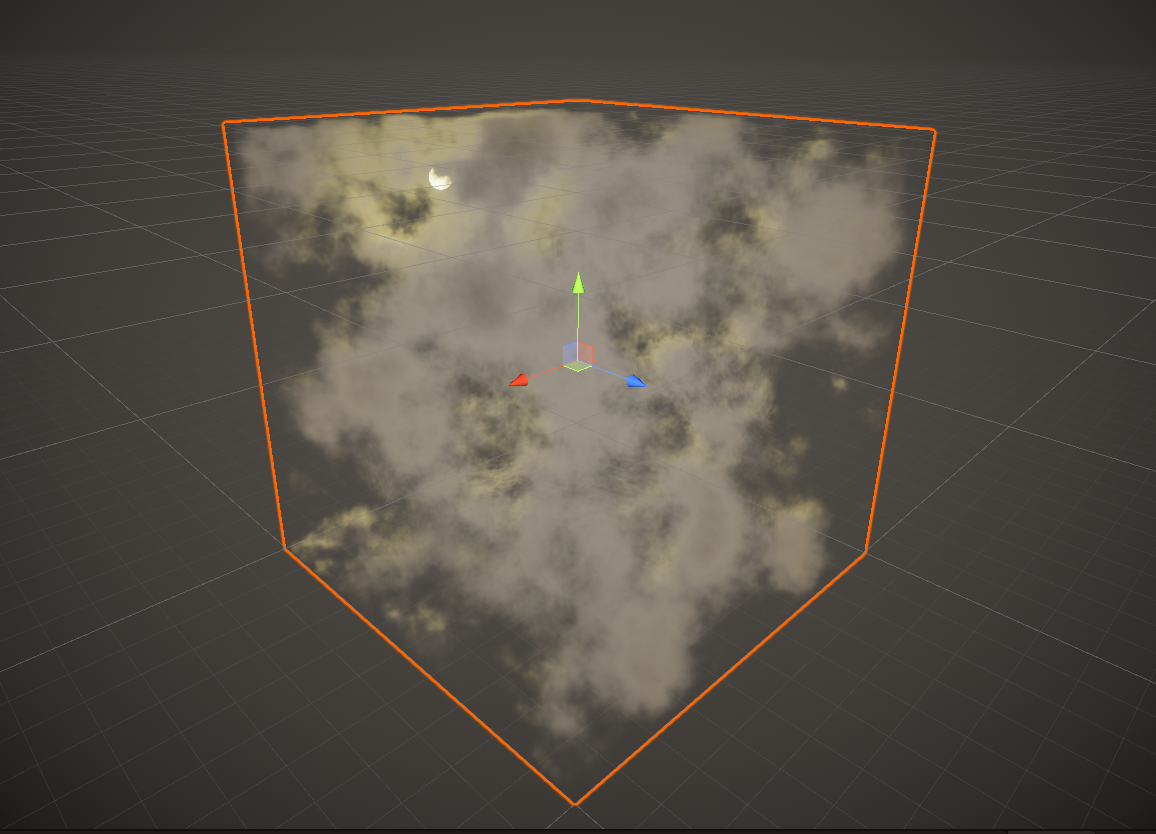
\includegraphics[width=\linewidth]{unity captures/prototype5.PNG}
    \captionof{figure}{Prototype: Rendered image of directional sunlight implemented with \gls{lightmarching}.}
    \label{img:captures:prototype5}
\end{figure}

\clearpage
\subsection{Final Prototype}
All put together and after quite some effort and experimenting, the rendered scene looks quite convincing. 
\\
Free assets from the Unity Asset Store were used for trees\footnote[1]{https://assetstore.unity.com/packages/3d/vegetation/speedtree/free-speedtrees-package-29170} and rocks\footnote[2]{https://assetstore.unity.com/packages/3d/environments/landscapes/photoscanned-moutainsrocks-pbr-130876}.

\begin{figure}[H]
    \centering
    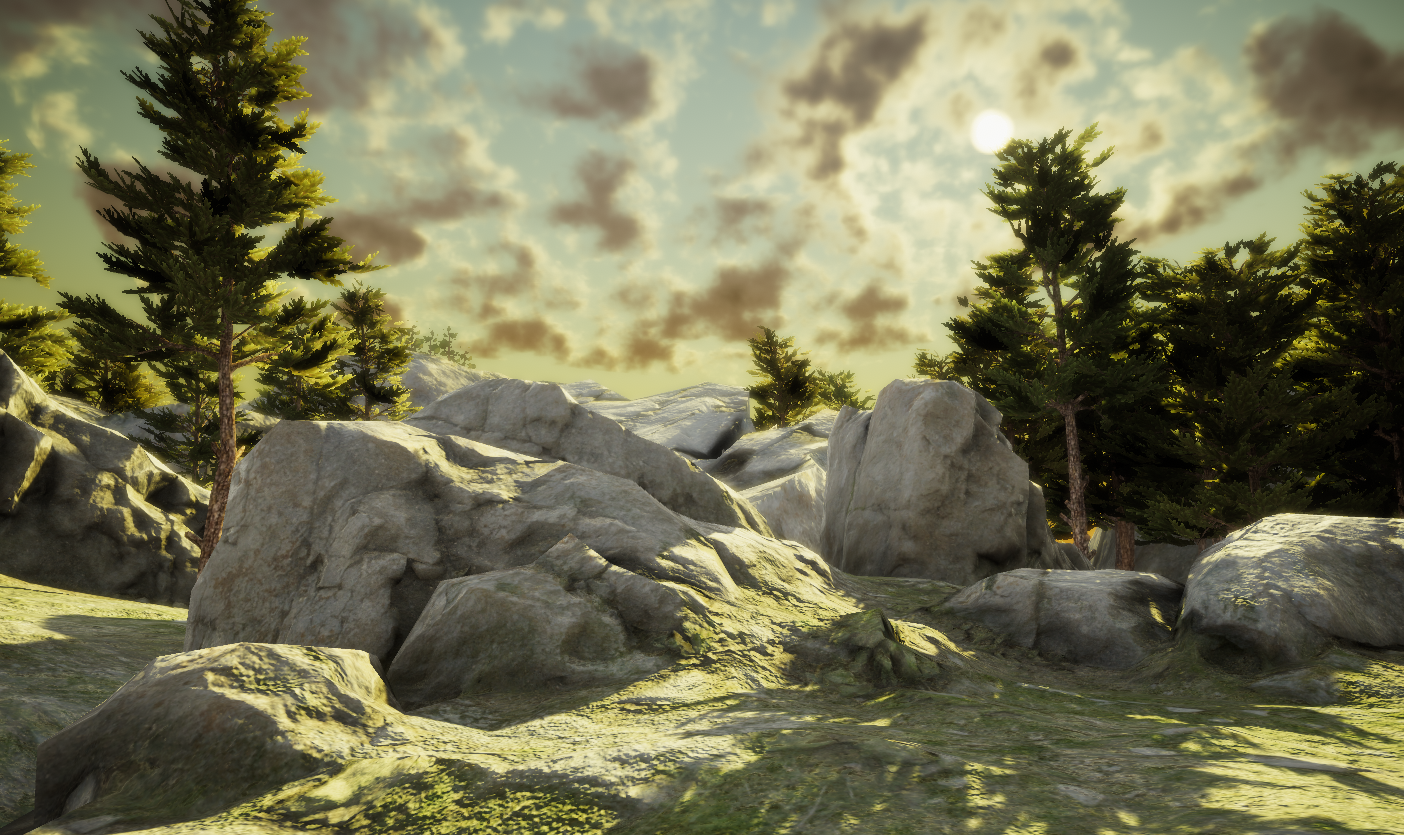
\includegraphics[width=\linewidth]{unity captures/final_dusk.PNG}
    \captionof{figure}{Prototype: Rendered image of the final prototype (afternoon scene).}
    \label{img:captures:prototype_final:afternoon}
\end{figure}

\clearpage
\noindent
To demonstrate the capability of the shader in its prototype state, here are some variations of it. The are no code changes in-between the rendered images, the only things that changed are the shader's \gls{parameters} and Unity Editor lighting settings and colors.

\begin{figure}[H]
    \centering
        \begin{minipage}{0.47\linewidth}
            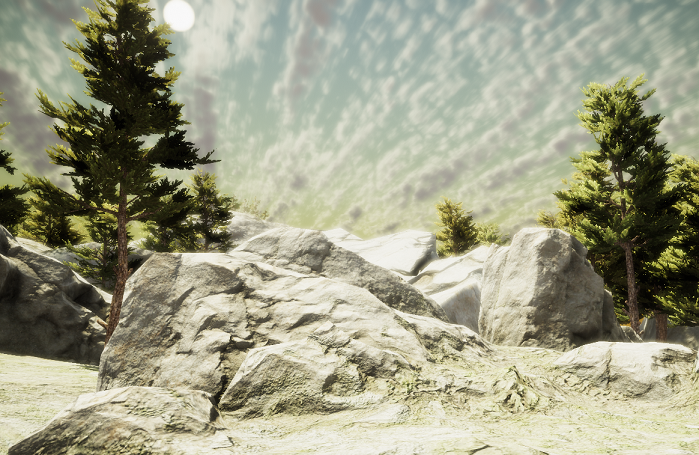
\includegraphics[width=\linewidth]{unity captures/final doc/final_day_small.PNG}
            \captionof{figure}{Prototype: Rendered day scene.}
            \label{img:captures:prototype_final:day}
        \end{minipage}
    \hfill
        \begin{minipage}{0.47\linewidth}
            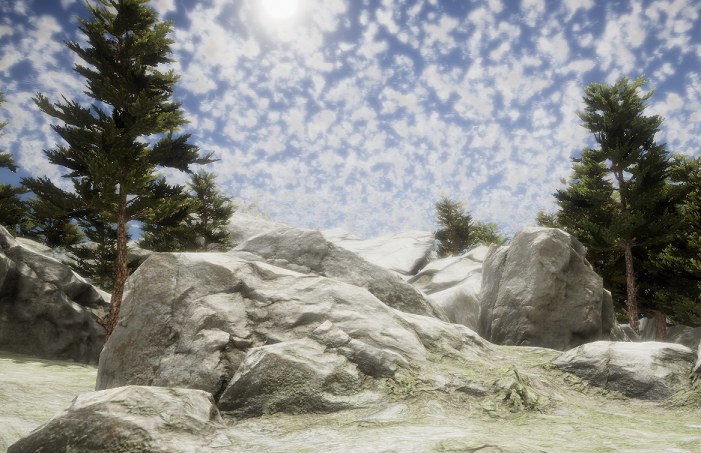
\includegraphics[width=\linewidth]{unity captures/final doc/final_puffy_small.PNG}
            \captionof{figure}{Prototype: Rendered puffy sky scene.}
            \label{img:captures:prototype_final:puffy}
        \end{minipage}
\end{figure}

\begin{figure}[H]
    \centering
        \begin{minipage}{0.47\linewidth}
            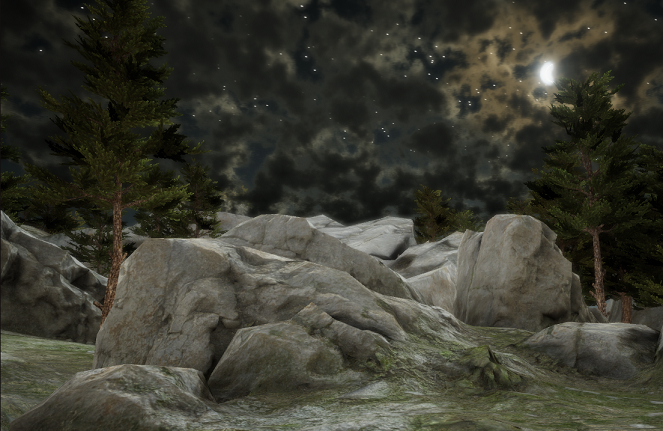
\includegraphics[width=\linewidth]{unity captures/final doc/final_night_small.PNG}
            \captionof{figure}{Prototype: Rendered night scene.}
            \label{img:captures:prototype_final:night}
        \end{minipage}
    \hfill
        \begin{minipage}{0.47\linewidth}
            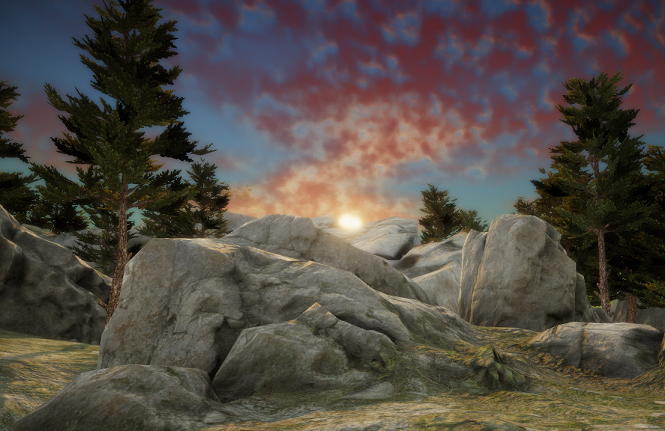
\includegraphics[width=\linewidth]{unity captures/final doc/final_sunset_small.PNG}
            \captionof{figure}{Prototype: Rendered sunset scene.}
            \label{img:captures:prototype_final:sunset}
        \end{minipage}
\end{figure}

\begin{figure}[H]
    \centering
        \begin{minipage}{0.47\linewidth}
            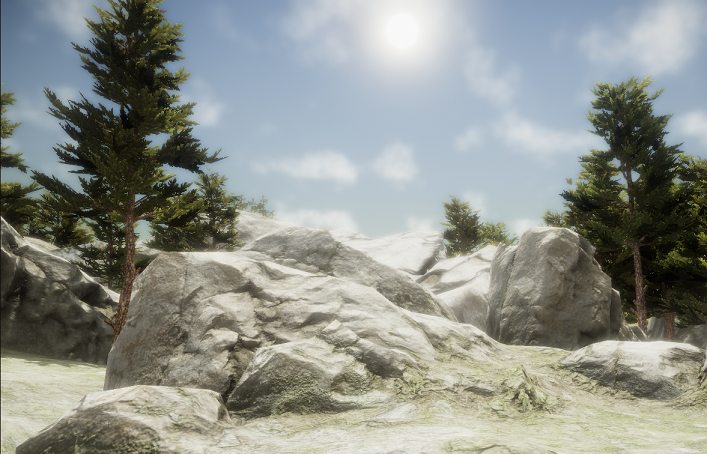
\includegraphics[width=\linewidth]{unity captures/final doc/final_clear_small.PNG}
            \captionof{figure}{Prototype: Rendered clear sky scene.}
            \label{img:captures:prototype_final:clear}
        \end{minipage}
    \hfill
        \begin{minipage}{0.47\linewidth}
            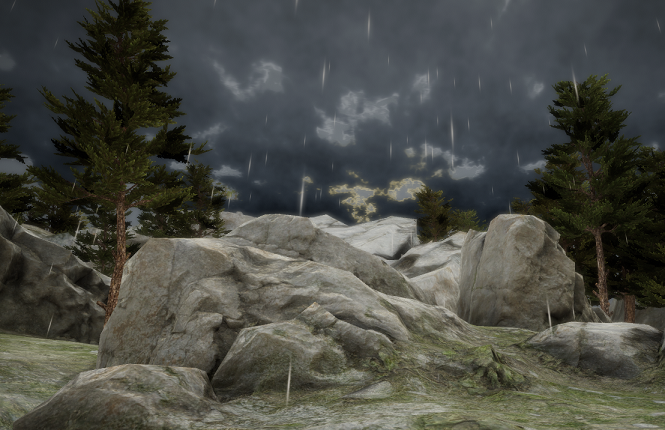
\includegraphics[width=\linewidth]{unity captures/final doc/final_stormy_small.PNG}
            \captionof{figure}{Prototype: Rendered stormy scene.}
            \label{img:captures:prototype_final:stormy}
        \end{minipage}
\end{figure}

\clearpage
\subsubsection{Additional Masking}
Technically, by multiplying both noise function values in \lstinline[language=HLSL]{sampleDensity()}, they already mask each other. In certain types of cloud formations, an additional masking needs to be applied in order to create a cloudscape that does not expand over the whole container cube.
This is done by feeding a mask texture into the shader, for which the cube's UV coordinates are used to sample the grey value of the texture at that position.

\begin{figure}[H]
    \centering
    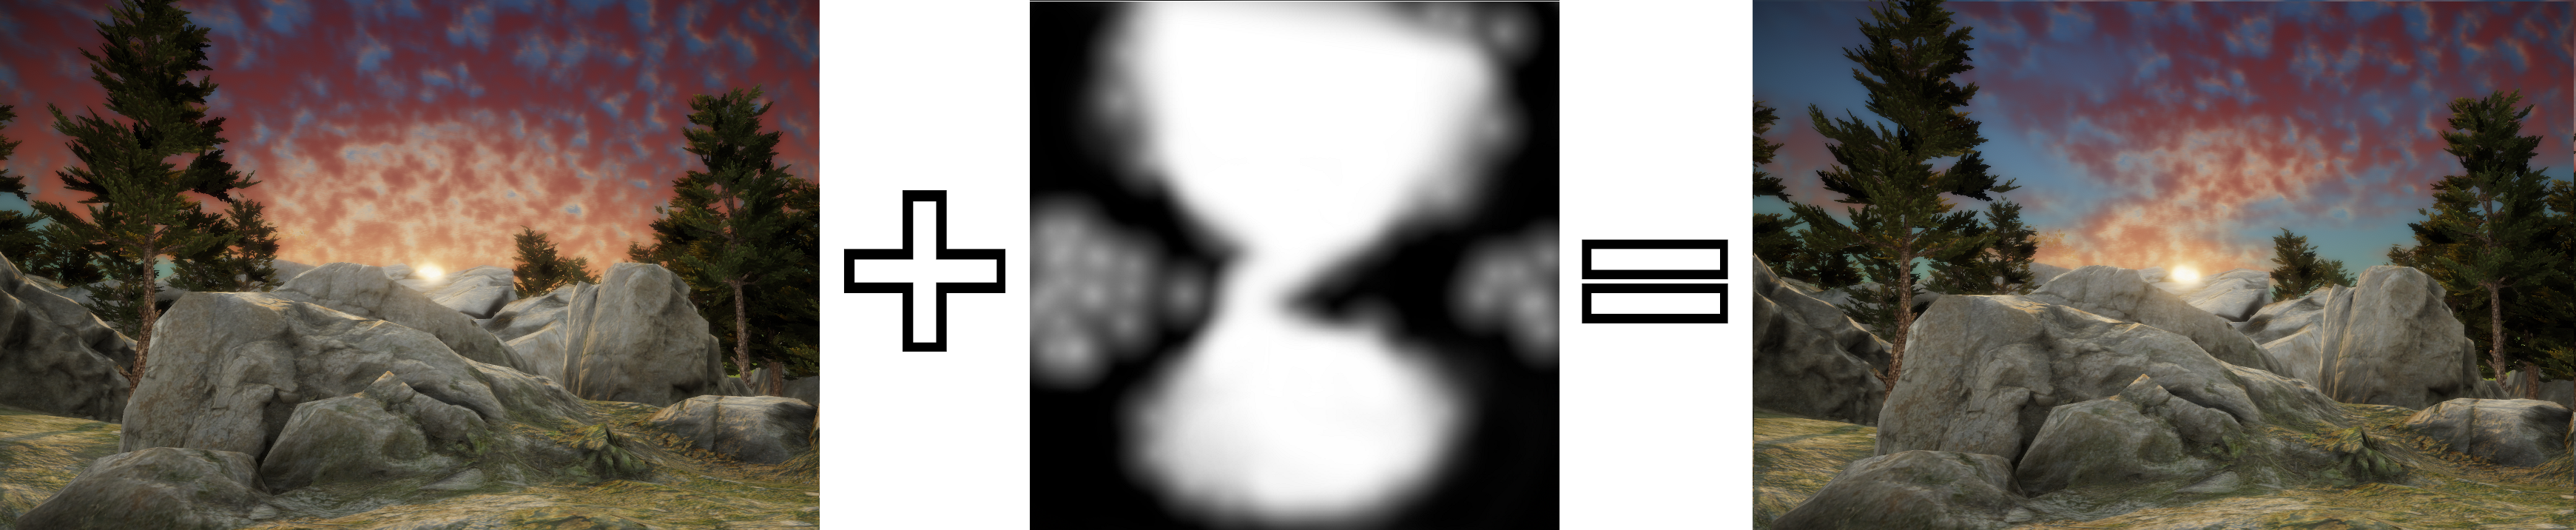
\includegraphics[width=\linewidth]{comparisons/masking.png}
    \captionof{figure}{Prototype: Masking with UV coordinates of the container cube.}
    \label{img:camparisons:masking}
\end{figure}

\clearpage
\subsection{Realism Check}
\label{section:prototypes:realismcheck}
While the prototypes in \autoref{img:captures:prototype_final:day} to \autoref{img:captures:prototype_final:stormy} do look realistically to a certain degree, it is still essential to have some sort of measurable factor with which the rendered images can be compared to real clouds.
Some factor that ultimately shows how \textit{real} the rendered clouds actually are, apart from the human eye interpretation.

\subsubsection{Objective interpretation}
Before expanding on how to measure the realism of the cloud shader's output, it seems important to objectively identify the capabilities of it first.
As originally stated in \sectionref{section:clouds-in-games}, the desired look of the clouds was that of the genus \textit{cumulus}.
\\
In the following subsection, each rendered image is compared to a real-life photograph, putting them into a objectively comparable state to reality.

\clearpage
\subsubsection{Real Life Comparison}
In all the following comparison images, the left images are photographic references and the right side images are rendered in Unity Engine.
\emptyline
\autoref{img:captures:prototype_final:day} and \autoref{img:captures:prototype_final:puffy} both resemble cirrocumulus and altocumulus clouds.
The cirrocumulus clouds are similar to altocumulus clouds, but they form at higher altitude and are significantly smaller, yet equally puffy.
\\
\autoref{img:captures:prototype_final:night} and \autoref{img:captures:prototype_final:sunset} also show the distinctive cotton-like pattern of the altocumulus genus.
When comparing to an actual photograph, there are only few differences.
\emptyline
By adjusting the scale of the shader, the clouds can be made smaller. In the following comparison, the directional \gls{lightmarching} has been turned down to a minimum so the light would look more wan. 

\begin{figure}[H]
    \centering
    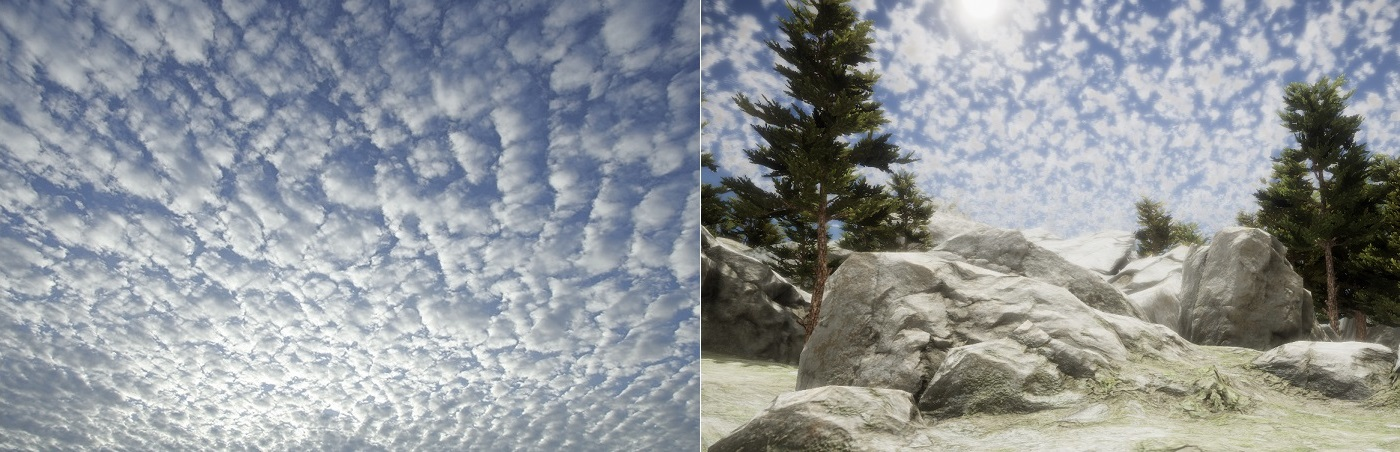
\includegraphics[width=\linewidth]{comparisons/compare_altocumulus.jpg}
    \captionof{figure}{Comparison: photographic reference \protect\cite{img:campare:altocumulus} versus the rendered image.}
    \label{img:comparisons:altocumulus}
\end{figure}

\noindent
The night-time comparison displays how the different color of the \gls{sunlightforwarding} can impact the scene.

\begin{figure}[H]
    \centering
    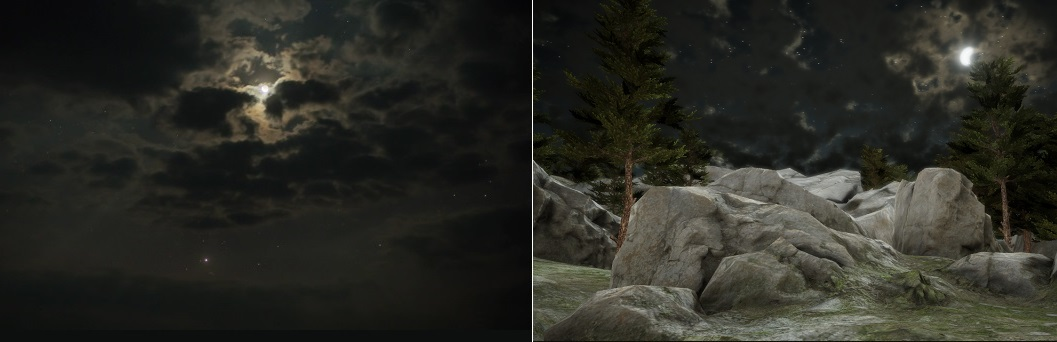
\includegraphics[width=\linewidth]{comparisons/compare_altocumulus_night.jpg}
    \captionof{figure}{Comparison: photographic reference \protect\cite{img:campare:altocumulus:night} versus the rendered image (at night).}
    \label{img:comparisons:altocumulus:night}
\end{figure}

\clearpage
\noindent
In \autoref{img:captures:prototype_final:sunset}, it is very clearly recognizable that the \gls{parameters} of the shader can heavily influence the lighting and illumination of the clouds.
Unfortunately, the difference of details and density is fairly discernable from reality and the desired appearance is not fully achieved.

\begin{figure}[H]
    \centering
    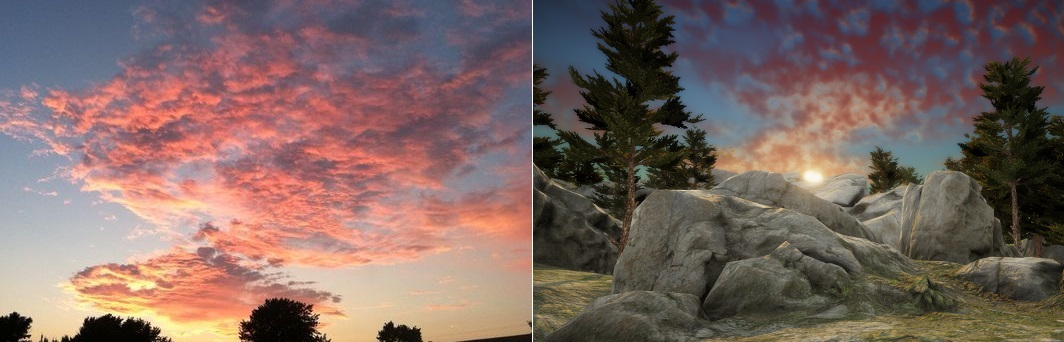
\includegraphics[width=\linewidth]{comparisons/compare_altocumulus_sunset.jpg}
    \captionof{figure}{Comparison: photographic reference \protect\cite{img:campare:altocumulus:sunset} versus the rendered image (at sunset).}
    \label{img:camparisons:altocumulus:sunset}
\end{figure}

\noindent
Finally, \autoref{img:captures:prototype_final:stormy} represents clouds of the type \textit{nimbostratus}, which form in low altitude and are dense and dark, often rainy.


\begin{figure}[H]
    \centering
    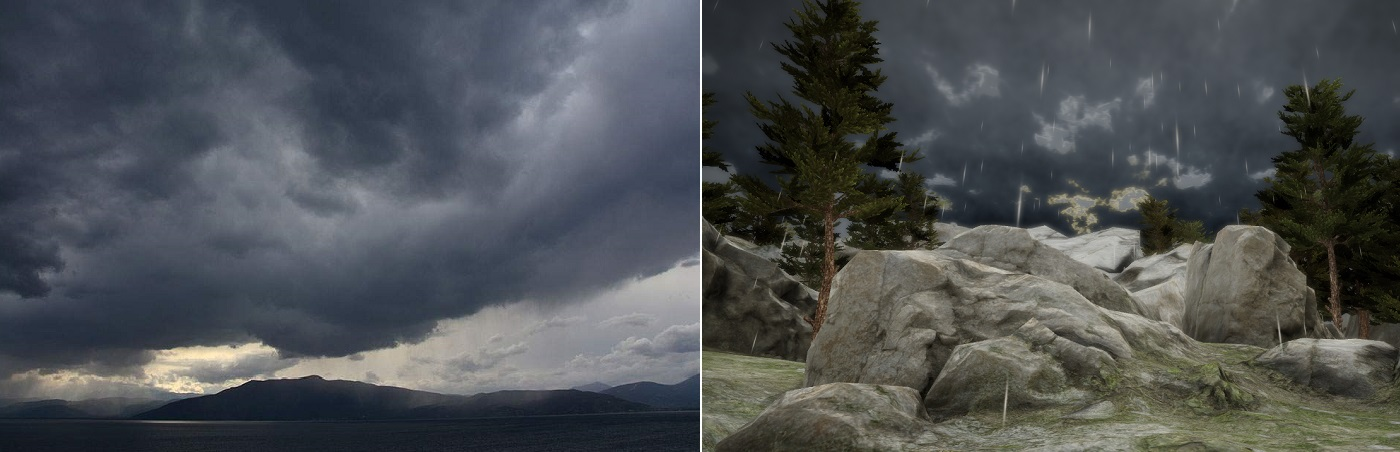
\includegraphics[width=\linewidth]{comparisons/compare_altocumulus_stormy.jpg}
    \captionof{figure}{Comparison: photographic reference \protect\cite{img:campare:altocumulus:stormy} versus the rendered image (stormy).}
    \label{img:camparisons:altocumulus:stormy}
\end{figure}

\noindent
With the \gls{sunlighttransmittance} being a bright yellow in the rendered image, an attempt was made to make the sun shine through the distant rainy clouds, like in the photographic reference. Since the cloud shader does not end before the horizon, the resulting effect is rather imperceptible.

\clearpage
\subsubsection{Convolutional Neural Network}
Given there is a \gls{cnn} (CNN) that is able to classify images of the sky, the weather or clouds into descriptive labels or even genera of cloud formations, then one could just seed those rendered images into the CNN and verify whether the results are truthfully showing "real" clouds.
Of course, this is heavily dependent of how well the CNN was trained.

\subsubsection{Generative Adversarial Network}
A similar approach to the \gls{cnn} is a  \gls{gan} (GAN) setup. It describes two neural networks, which contest with each other in a cat-and-mouse game: The \textit{generative} network tries to imitate the training set by generating artificial photographs with many realistic characteristics, while the \textit{discriminative} network tries to tell whether the generated images are fake or not.
\\
With this method, the rendered cloud images could be passed through the discriminative neural network to see if at least the network thinks the images are of real clouds.

\subsubsection{Histogram Comparison}
The \textit{\gls{histogram}} is a graphical representation of data like brightness or color distribution of a given photograph.
When extracting the color \gls{histogram}s of the real photograph and the one of the rendered image, they could be compared and rated how different in color they are.

\subsubsection{Professional Meteorological Assessment}
Another viable solution is to let a professional meteorologist inspect and rate the rendered images and judge the realism of the depicted scenarios, which should reveal if the rendered clouds could actually form and exist in reality.

\clearpage
\subsection{Performance}
With the current implementations of \gls{raymarching} and \gls{lightmarching}, the performance of the shader is heavily dependent on the number of samples $N$ and $L$ taken along the rays.
With a container cube the size of 400x200 pixel in screen-space (which is a relatively small box of clouds), the \gls{gpu} load is already enormously large. 
Here, the number of noise samplings $N_{total}$ is calculated as follows. The values for $N$ and $L$ are both set to a minimum of 25, since it seemed to achieve the best looking results during prototyping.
$$ 
\begin{array}{l}
    w = 400, h = 200\\
    N = 25, L = 25\\ \\
    N_{total} = w * h * N * L = 5 * 10^7
\end{array}
$$

\noindent
So for a single frame, the number of times the noise function is called for this example is just about fifty million times. This inconceivably high number makes the current implementation desperately needy of optimization.

\subsubsection{Optimization Attempts}
\paragraph{Compute Shader}
The fact that the noise function needs to be sampled so often may not even be the issue, but rather that the noise texture needs to be calculated again each time.
Therefore, the idea arose to precalculate the 3D noise volume and feed it to the shader at runtime, in the form of a 3D texture cube.
\\
For this, a \gls{computeshader} was created with the attempt to generate said texture.
Unfortunately, all experiments with \gls{computeshader}s were unsuccessful, as there is only very little documentation about 3D texture-generating \gls{computeshader}s for Unity Editor.
This attempt was therefore abandoned.

\paragraph{Early Exits}
For some functions and loops, early exit conditions can speed up the shader. As an example in \autoref{lst:shader:prototype:raylightmarching}, which describes \gls{raymarching} combined with \gls{lightmarching}, the light does not need to be calculated when there is no cloud.
The following little extension should fix that issue.
\begin{lstlisting}[language=HLSL]
if (density <= 0) {
    return float2(0, 0);
}
\end{lstlisting}

\noindent
Instead of checking if \lstinline[language=HLSL]{density} is smaller or equal to zero, a very small threshold could be used as well.
It is noteworthy that a number larger than zero can create edges on thin clouds, as the abrupt reduction in density may be visible.
\clearpage

\printnoidxglossary 
\clearpage
\printbibliography[heading=bibintoc]
\clearpage
\phantomsection
\addcontentsline{toc}{section}{Listings}
\phantomsection
\addcontentsline{toc}{subsection}{Figures}
\listoffigures
\clearpage
\phantomsection
\addcontentsline{toc}{subsection}{Code Listings}
\lstlistoflistings

\end{document}
